\documentclass[12pt]{article}

\usepackage[]{graphicx}
\usepackage[]{color}
\usepackage{alltt}

\newcommand{\mytitle}{Monte Carlo Methods and Random Sampling}
\newcommand{\myname}{Nikolai German}
\newcommand{\mysupervisor}{Dr. Ludwig Bothmann}

\usepackage[a4paper, width = 160mm, top = 35mm, bottom = 30mm, 
bindingoffset = 0mm]{geometry}
\usepackage[utf8]{inputenc}
\usepackage{ragged2e}
\usepackage{xcolor}
\usepackage[round, comma]{natbib}
\usepackage{fancyhdr}
\newcommand{\changefont}{%
    \fontsize{8}{11}\selectfont
}
\usepackage{hyperref}
\hypersetup{
  colorlinks = true,
  linkcolor = black,
  urlcolor = black,
  citecolor = black}
\pagestyle{fancy}
\fancyhead{}
\fancyhead[R]{\changefont{\mytitle}}
\fancyfoot{}
\fancyfoot[R]{\thepage}
\setlength{\headheight}{14.5pt}
\setlength{\parindent}{0pt}
\interfootnotelinepenalty = 10000

\usepackage{amsthm}
\usepackage{algorithm}
\usepackage{algpseudocode}
\usepackage{mathtools}  % amsmath with extensions
\usepackage{amsfonts}  % (otherwise \mathbb does nothing)
\usepackage{subcaption}

%\newtheorem{theorem}{Theorem}[section]
%\newtheorem{corollary}{Corollary}[theorem]
%\newtheorem{lemma}[theorem]{Lemma}
%\newtheorem{example}{Example}[section]
%\theoremstyle{definition}
%\newtheorem{definition}{Definition}[section]

\usepackage{apxproof}
\renewcommand{\appendixprelim}[1]{}
\newtheoremrep{theorem}{Theorem}[section]
\newtheoremrep{corollary}{Corollary}[theorem]
\newtheoremrep{lemma}[theorem]{Lemma}
\newtheorem{example}{Example}[section]
\theoremstyle{definition}
\newtheorem{definition}{Definition}[section]


% ------------------------------------------------------------------------------
% MAIN -------------------------------------------------------------------------
% ------------------------------------------------------------------------------
\IfFileExists{upquote.sty}{\usepackage{upquote}}{}
\begin{document}

% FRONT PAGE -------------------------------------------------------------------
 
\begin{titlepage}
\begin{center}
    
\LARGE
Seminar Paper
    
\vspace{0.5cm}
      
\rule{\textwidth}{1.5pt}
\LARGE
\textbf{\mytitle}
\rule{\textwidth}{1.5pt}
   
\vspace{0.5cm}
      
\large
Department of Statistics \\
Ludwig-Maximilians-Universität München 

\vfill

\Large
\textbf{\myname}

\vfill

\large
Munich, July 6\textsuperscript{th}, 2025
      
\vfill


\includegraphics[width = 0.4\textwidth]{sigillum.png}

\vfill

\normalsize
Submitted in partial fulfillment of the requirements for the degree of B. Sc.
\\

Supervised by \mysupervisor

\end{center}
\end{titlepage}

% CONTENTS ---------------------------------------------------------------------

\pagenumbering{Roman}
\newpage

\begin{abstract}
Monte Carlo methods provide essential computational tools for solving high-dimensional integration and sampling problems that are analytically intractable. This paper presents a comprehensive treatment of Monte Carlo techniques, beginning with fundamental integration principles and the curse of dimensionality that motivates probabilistic approaches. We systematically develop key sampling algorithms including the inversion method, Box-Muller transformation, and acceptance-rejection techniques, providing both basic and adaptive variants. We present different variance reduction strategies: most importantly importance sampling (direct and self-normalized variants). We complement pseudo-random approaches with quasi-Monte Carlo methods for improved convergence rates. Practical effectiveness is demonstrated through classical applications including $\pi$ approximation and rare event estimation in financial risk models, where importance sampling achieves dramatic efficiency gains over standard approaches. The paper concludes with a critical assessment of advantages and limitations, along with an outlook toward advanced methods including sequential importance sampling and Markov Chain Monte Carlo.
\end{abstract}

\newpage
\tableofcontents

%%%% if you would want to include material overview
%%%% use one of the following in addition
% \newpage
% \listoffigures
% \newpage
% \listoftables
\newpage

% CHAPTERS ---------------------------------------------------------------------

\pagenumbering{arabic}
    
\section{Introduction}
\label{intro}
Monte Carlo methods represent a broad class of computational algorithms that rely on repeated random sampling to obtain numerical results. These methods have become indispensable tools across numerous fields, from physics and engineering to finance and machine learning, particularly when dealing with complex, high-dimensional problems that defy analytical solutions.

The power of Monte Carlo approaches lies in their ability to transform difficult mathematical problems into statistical sampling problems. Rather than attempting to solve equations directly, these methods generate random samples from probability distributions and use statistical inference to extract the desired information.

This paper examines the theoretical foundations and practical applications of Monte Carlo methods, with particular emphasis on integration techniques. We begin by introducing the core concepts that form the foundation of this methodology. For improved readability, formal proofs of all theorems are provided in the appendix. Some of the examples and implementations discussed later on, can also be found in greater detail on \href{https://nikogerman.github.io/Seminar/index.html}{\color{blue}GitHub Pages}.


\paragraph{Monte Carlo method}
The Monte Carlo method originated in the mid-1940s during the Manhattan Project, primarily through the work of Stanislaw Ulam, who conceived the basic idea, and John von Neumann, who developed the mathematical framework. Nicholas Metropolis later contributed to its development and suggested the name. The method emerged from their need to solve complex mathematical problems in nuclear physics that involved high-dimensional integrals too complicated for analytical solutions. Their innovation was to use random sampling to approximate these mathematical calculations, creating what became known as the Monte Carlo method.

\cite{lemieux_monte_2009} summarizes the method as:
\begin{quote}
The use of random sampling as a tool to produce
observations on which statistical inference can be performed to extract information about a system.
\end{quote}

\paragraph{Monte Carlo integration}
Monte Carlo integration estimates integrals of the form
$$
I(f) = \int_{\mathcal{D}}f(x)dx 
$$
by sampling points uniformly at random from the domain $\mathcal{D}$, evaluating the function $f$ at these sample points, and using the sample average to approximate the integral. This approach becomes particularly advantageous in high-dimensional settings where traditional quadrature methods suffer from the curse of dimensionality. Chapter \ref{sampling} discusses techniques for generating samples from various distributions, while Chapter \ref{variance-control} explores methods to improve the efficiency of Monte Carlo integration through variance reduction. The theoretical foundations and detailed implementation of these integration techniques are covered in Chapter \ref{MC-Integration}.

\paragraph{Monte Carlo simulation}
Monte Carlo simulation generates samples from complex random variables $Y = \varphi(X)$ by first sampling the input variables $X$ and then applying the transformation $\varphi$. This sampling-based approach allows us to study the statistical properties of $Y$ even when direct sampling or analytical solutions are intractable. The practical implementation relies on efficient sampling algorithms (Chapter \ref{sampling}) and can often benefit from variance reduction strategies (Chapter \ref{variance-control}) to improve computational efficiency. While Monte Carlo simulation shares the fundamental sampling principles with Monte Carlo integration (Chapter \ref{MC-Integration}), it focuses on generating realizations from complex distributions rather than estimating integrals. Although \cite{lemieux_monte_2009} shows that simulation problems are integration problems and vice versa, we will use the distinction for the sake of clarity.

\paragraph{Quasi-Monte Carlo methods}
Quasi-Monte Carlo methods, examined in detail in Chapter \ref{QMC}, generate deterministic point sets $\{u_1, \dots, u_n\}$ in $[0,1]^d$ that are more uniformly distributed than random samples. These low-discrepancy sequences provide better coverage of the unit hypercube, often achieving faster convergence rates than standard Monte Carlo methods for smooth integrands.

\paragraph{Random Numbers}
Random number generation forms the foundation of Monte Carlo methods. As we will demonstrate in subsequent chapters, we can generate random quantities from virtually any distribution by starting with uniform random numbers, making $U(0,1)$ the fundamental building block for all sampling methods.

In practice, computational applications rely on pseudo-random number generators (see Appendix~\ref{appendix:rng} for an exemplary implementation). For the remainder of this work we assume access to a reliable algorithm $\texttt{RUNIF\_01}(n)$ that outputs $n$ independent and identically distributed random numbers following $U(0,1)$.

\cite{thomopoulos_essentials_2013, lemieux_monte_2009} provide good introductions into the properties and the construction of pseudo-random number generators.

\section{Monte Carlo Integration}
\label{MC-Integration}
In statistics and probabilistic machine learning, we frequently encounter integrals that cannot be solved analytically. A common form is:
\begin{equation}
\label{eq:mc-int}
I(\varphi) = \int \varphi(x)f(x) dx
\end{equation}
where $f(x)$ is a probability density function and $\varphi(x)$ is some function of interest.
Such integrals typically require numerical approximation methods.
The Monte Carlo approach to integration is based on a fundamental insight: if we can sample from the probability distribution $f(x)$, we can approximate the integral via the sample average. The Monte Carlo estimator is therefore defined as:
\begin{equation}
\label{eq:mc-estimator}
\hat{\mu}_n = \frac{1}{n} \sum_{i=1}^n \varphi(X_i) \quad \text{where} \quad X_1, \ldots, X_n \overset{\text{i.i.d.}}{\sim} f
\end{equation}
Integrals of the form shown in \eqref{eq:mc-int} commonly represent expectations under posterior distributions, marginal likelihoods, or normalization constants. This becomes clearer through the following examples, with $X \sim f$:
\begin{align*}
\varphi(x) = x &\quad \Rightarrow \quad I(\varphi) = \mathbb{E}_f[X] \\
\varphi(x) = \mathbb{I}(x \leq \gamma) &\quad \Rightarrow \quad I(\varphi) = F_X(\gamma) \\
\varphi(x) = 1 &\quad \Rightarrow \quad I(\varphi) = \int f(x)dx
\end{align*}

\begin{example}
\label{ex:sin}
    Consider the integral $I = \int_0^{\pi} \sin(x)\,dx$. The exact value is $I = 2$.
    Suppose we only have access to uniformly distributed random variables on the $[0, 1)$ interval.
    We therefore use substitution to transform the domain to $[0,1)$: $I = \pi \int_0^1 \sin(\pi \cdot u) du \approx \pi \cdot n^{-1} \sum_{i = 1}^n \sin(\pi \cdot U_i)$, where $U_i \overset{i.i.d.}{\sim} \text{Unif}(0,1)$ for all $i = 1,...,n$.
    
    \begin{figure}[h]
    \centering
    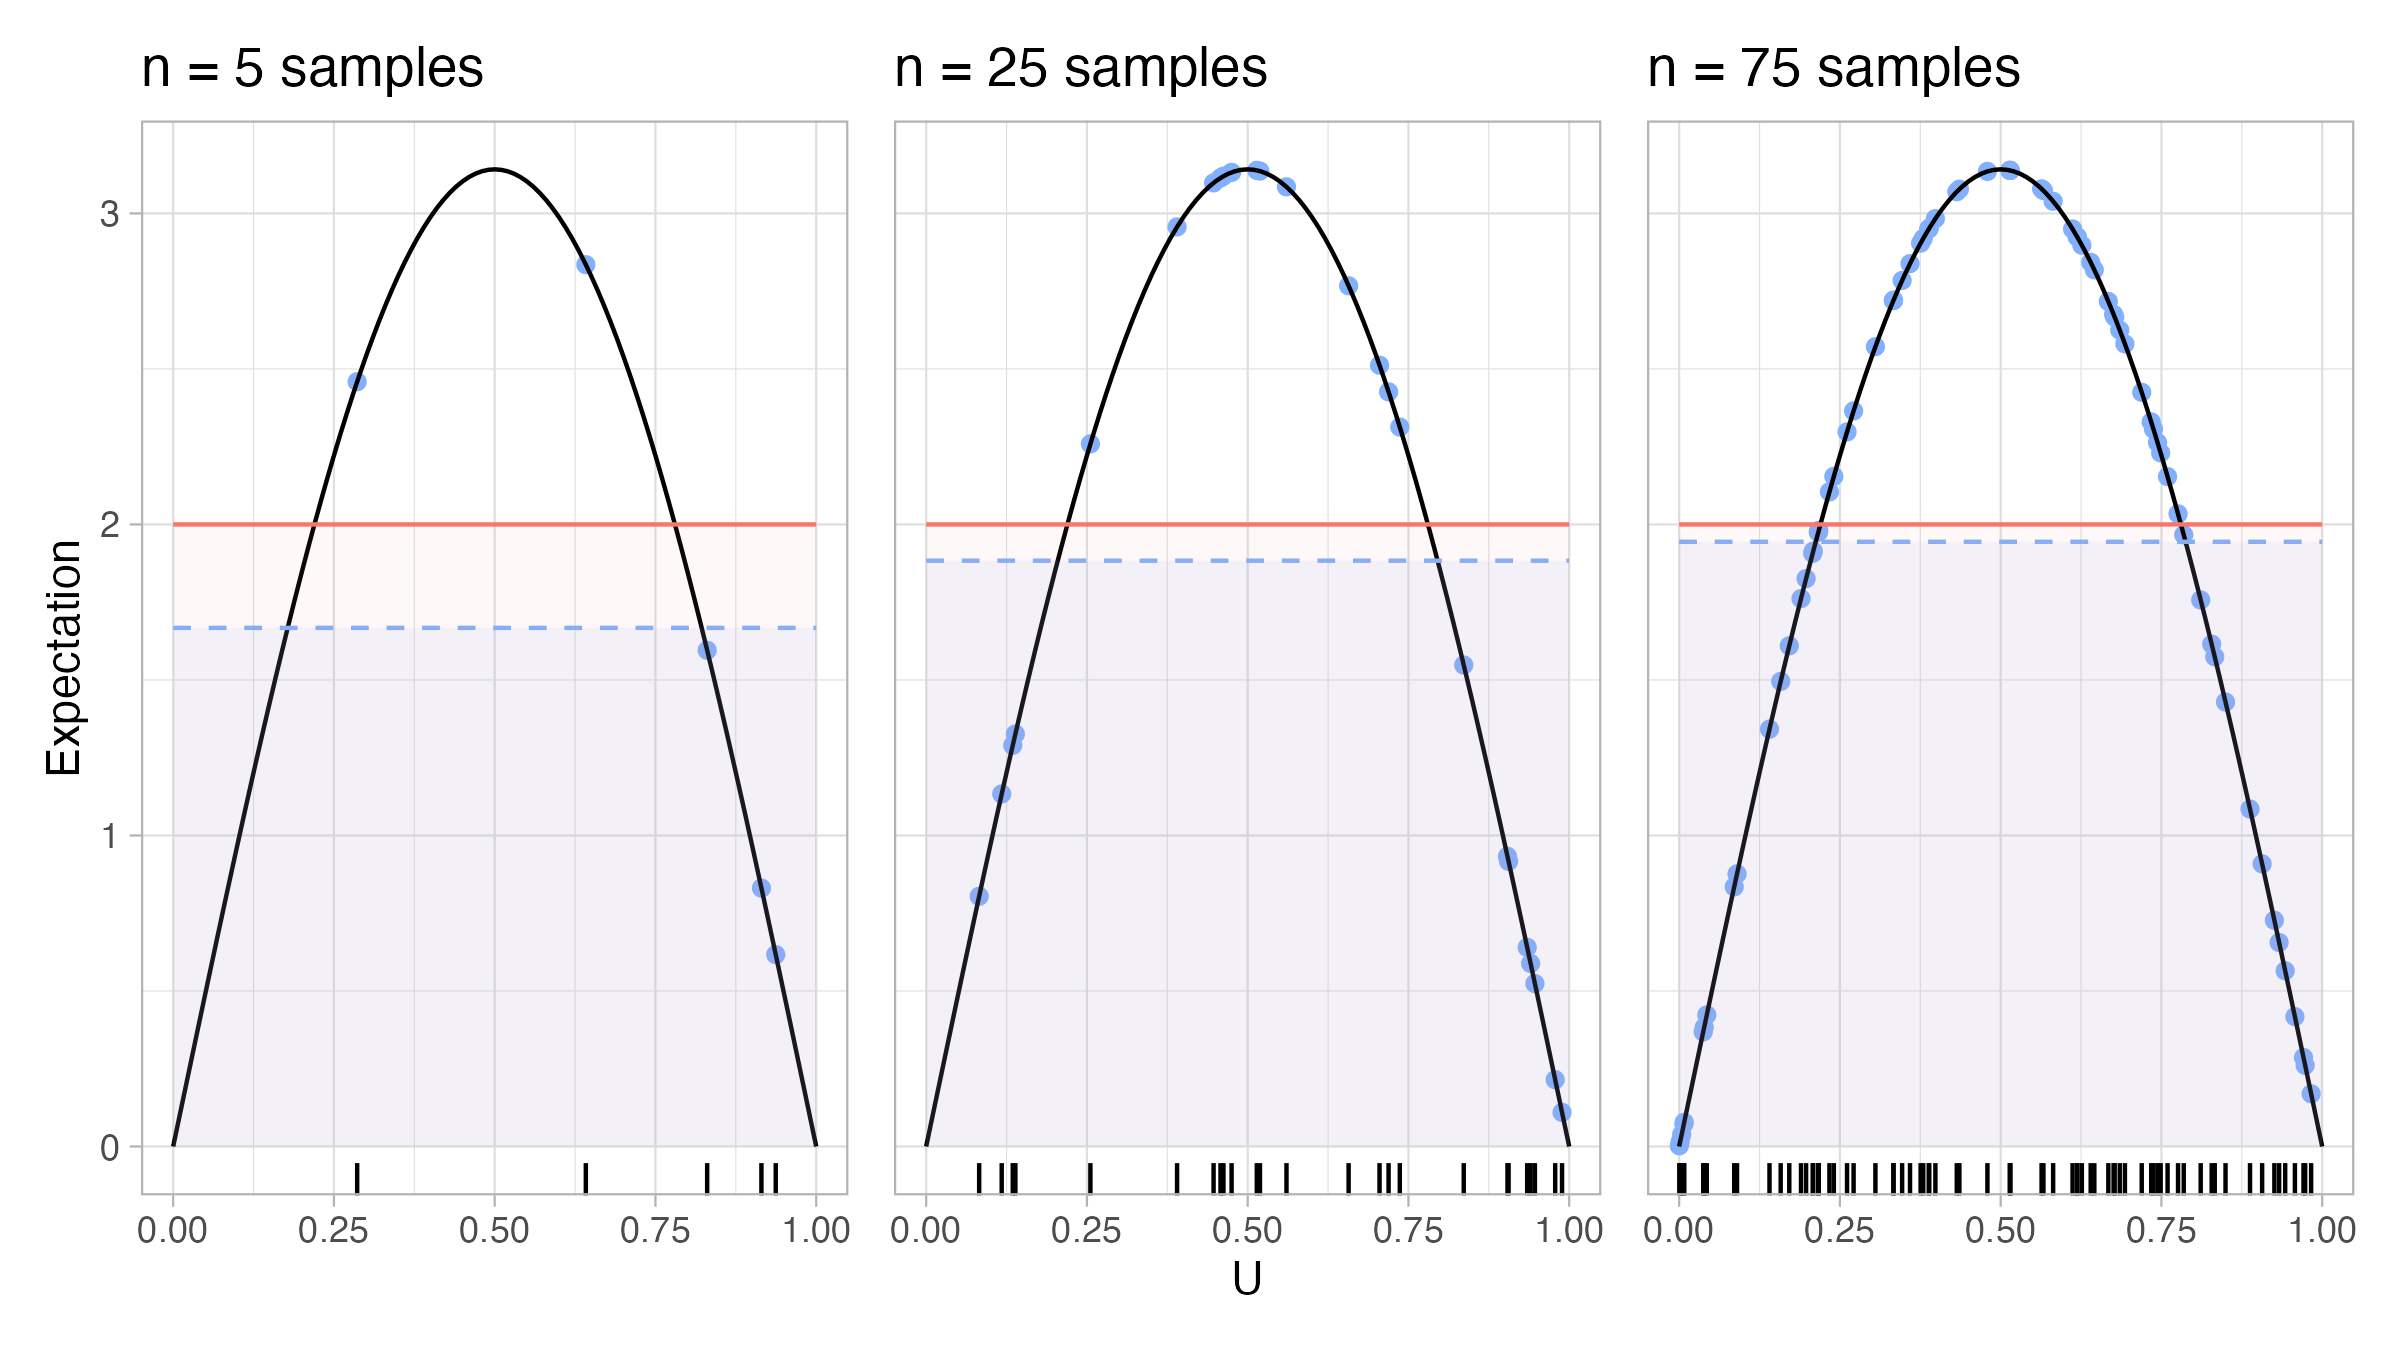
\includegraphics[width=.8\linewidth]{figures/mc-integration1.png}
    \caption{Monte Carlo approximation of $\int_0^{\pi} \sin(x)\,dx$ showing convergence to the true value of 2 as sample size increases. Generated using \href{https://github.com/NikoGerman/Seminar/blob/main/Notebooks/mc-integration.Rmd}{\texttt{mc-integration.Rmd}}.}
    \label{fig:mc-integration1}
\end{figure}
\end{example}

A comprehensive analysis of example \ref{ex:sin}, including convergence behavior and implementation details, can be found at \href{https://nikogerman.github.io/Seminar/Notebooks/mc-integration.html}{\texttt{mc-integration.html}}.

\subsection{Numerical integration and the curse of dimensionality}
An alternative to Monte Carlo integration is numerical integration, where traditional quadrature methods evaluate the integrand at regularly spaced grid points. While effective for low-dimensional problems, these methods suffer from the curse of dimensionality.
Maintaining accuracy requires $\tilde{N} = N^d$ function evaluations, where $N$ is the number of points per dimension and $d$ is the dimensionality. For example, a three-dimensional problem with $N=100$ points per dimension requires $100^3 = 10^6$ evaluations. Moreover, for the trapezoidal rule, the approximation error scales as $\mathcal{O}(\tilde{N}^{-2/d})$, making convergence prohibitively slow in high dimensions.
\begin{example}
\label{ex-cod}
Consider the $d$-dimensional integral
$$
\int_{[0,1]^d} f(\mathbf{x}) d\mathbf{x}
$$
where $f(\mathbf{x}) = 1$ if $x_i\in [0.4,0.6]$ for all $i=1,\dots,d$ and $f(\mathbf{x}) = 0$ otherwise.
Only $[0.2]^d$ of grid points contribute to the integral: 4\% for $d=2$, 0.032\% for $d = 5$, and less than $10^{-7}$\% for $d = 10$.
\end{example}
This \textit{curse of dimensionality} makes Monte Carlo methods particularly attractive, as their error depends only on $N$, not on dimensionality.

\subsection{Properties of the Monte Carlo Estimator}
The Monte Carlo estimator approximates the true expectation $\mu = \mathbb{E}_f[\varphi(X)]$ by averaging the function values $\varphi(X_i)$ over $n$ independent samples from the distribution $f$.

\begin{lemma}
\label{lemma-measurable-composition}
If $\varphi$ is a measurable function and $X_1, \ldots, X_n$ are i.i.d. random variables, then $\varphi(X_1), \ldots, \varphi(X_n)$ are also i.i.d. random variables.
\end{lemma}

\begin{proof}
This follows from the fact that the composition of a measurable function with a random variable is a random variable, and independence is preserved under measurable transformations.
\end{proof}

\begin{theoremrep}[Unbiasedness]
\label{theorem-unbiased}
The Monte Carlo estimator $\hat{\mu}_n$ is unbiased: 
\begin{equation}
    \mathbb{E}[\hat{\mu}_n] = \mu
\end{equation}
\end{theoremrep}

\begin{proof}
Assume $\mathbb{E}_f[\varphi(X)] = \mu$ exists. Then:
\begin{align*}
\mathbb{E}[\hat{\mu}_n] &= \mathbb{E}\left[\frac{1}{n}\sum_{i=1}^n\varphi(X_i)\right] \\
&= \frac{1}{n}\sum_{i=1}^n\mathbb{E}[\varphi(X_i)] \quad \text{(linearity of expectation)} \\
&= \frac{1}{n}\sum_{i=1}^n\mu \quad \text{(identical distribution)} \\
&= \mu
\end{align*}
\end{proof}

\begin{theoremrep}[Variance]
\label{theorem-variance}
The variance of the Monte Carlo estimator is 
\begin{equation}
    \text{Var}[\hat{\mu}_n] = \frac{\sigma^2}{n}
\end{equation}
where $\sigma^2 = \text{Var}_f[\varphi(X)]$.
\end{theoremrep}

\begin{proof}
Assume $\text{Var}_f[\varphi(X)] = \sigma^2 < \infty$. Then:
\begin{align*}
\text{Var}[\hat{\mu}_n] &= \text{Var}\left[\frac{1}{n}\sum_{i=1}^n\varphi(X_i)\right] \\
&= \frac{1}{n^2}\sum_{i=1}^n\text{Var}[\varphi(X_i)] \quad \text{(independence)} \\
&= \frac{1}{n^2} \cdot n \cdot \sigma^2 \quad \text{(identical distribution)} \\
&= \frac{\sigma^2}{n}
\end{align*}
\end{proof}

\begin{theorem}[Asymptotic Normality]
\label{theorem-clt}
Under regularity conditions, the Monte Carlo estimator satisfies:
\begin{equation}
\hat{\mu}_n - \mu \xrightarrow{d} \frac{1}{\sqrt{n}}\mathcal{N}(0, \sigma^2)
\end{equation}
\end{theorem}

This follows from the Central Limit Theorem\footnote{see Appendix \ref{appendix:clt}}. The key insight is that the estimation error decreases as $\mathcal{O}(n^{-1/2})$, independent of the dimension $d$ of the integration domain. This is the fundamental advantage of Monte Carlo methods over grid-based integration approaches in high-dimensional settings. Figure \ref{fig:mc-integration2} illustrates this convergence behavior by showing the estimation error for the integral from example \ref{ex:sin}.
\begin{figure}[h]
    \centering
    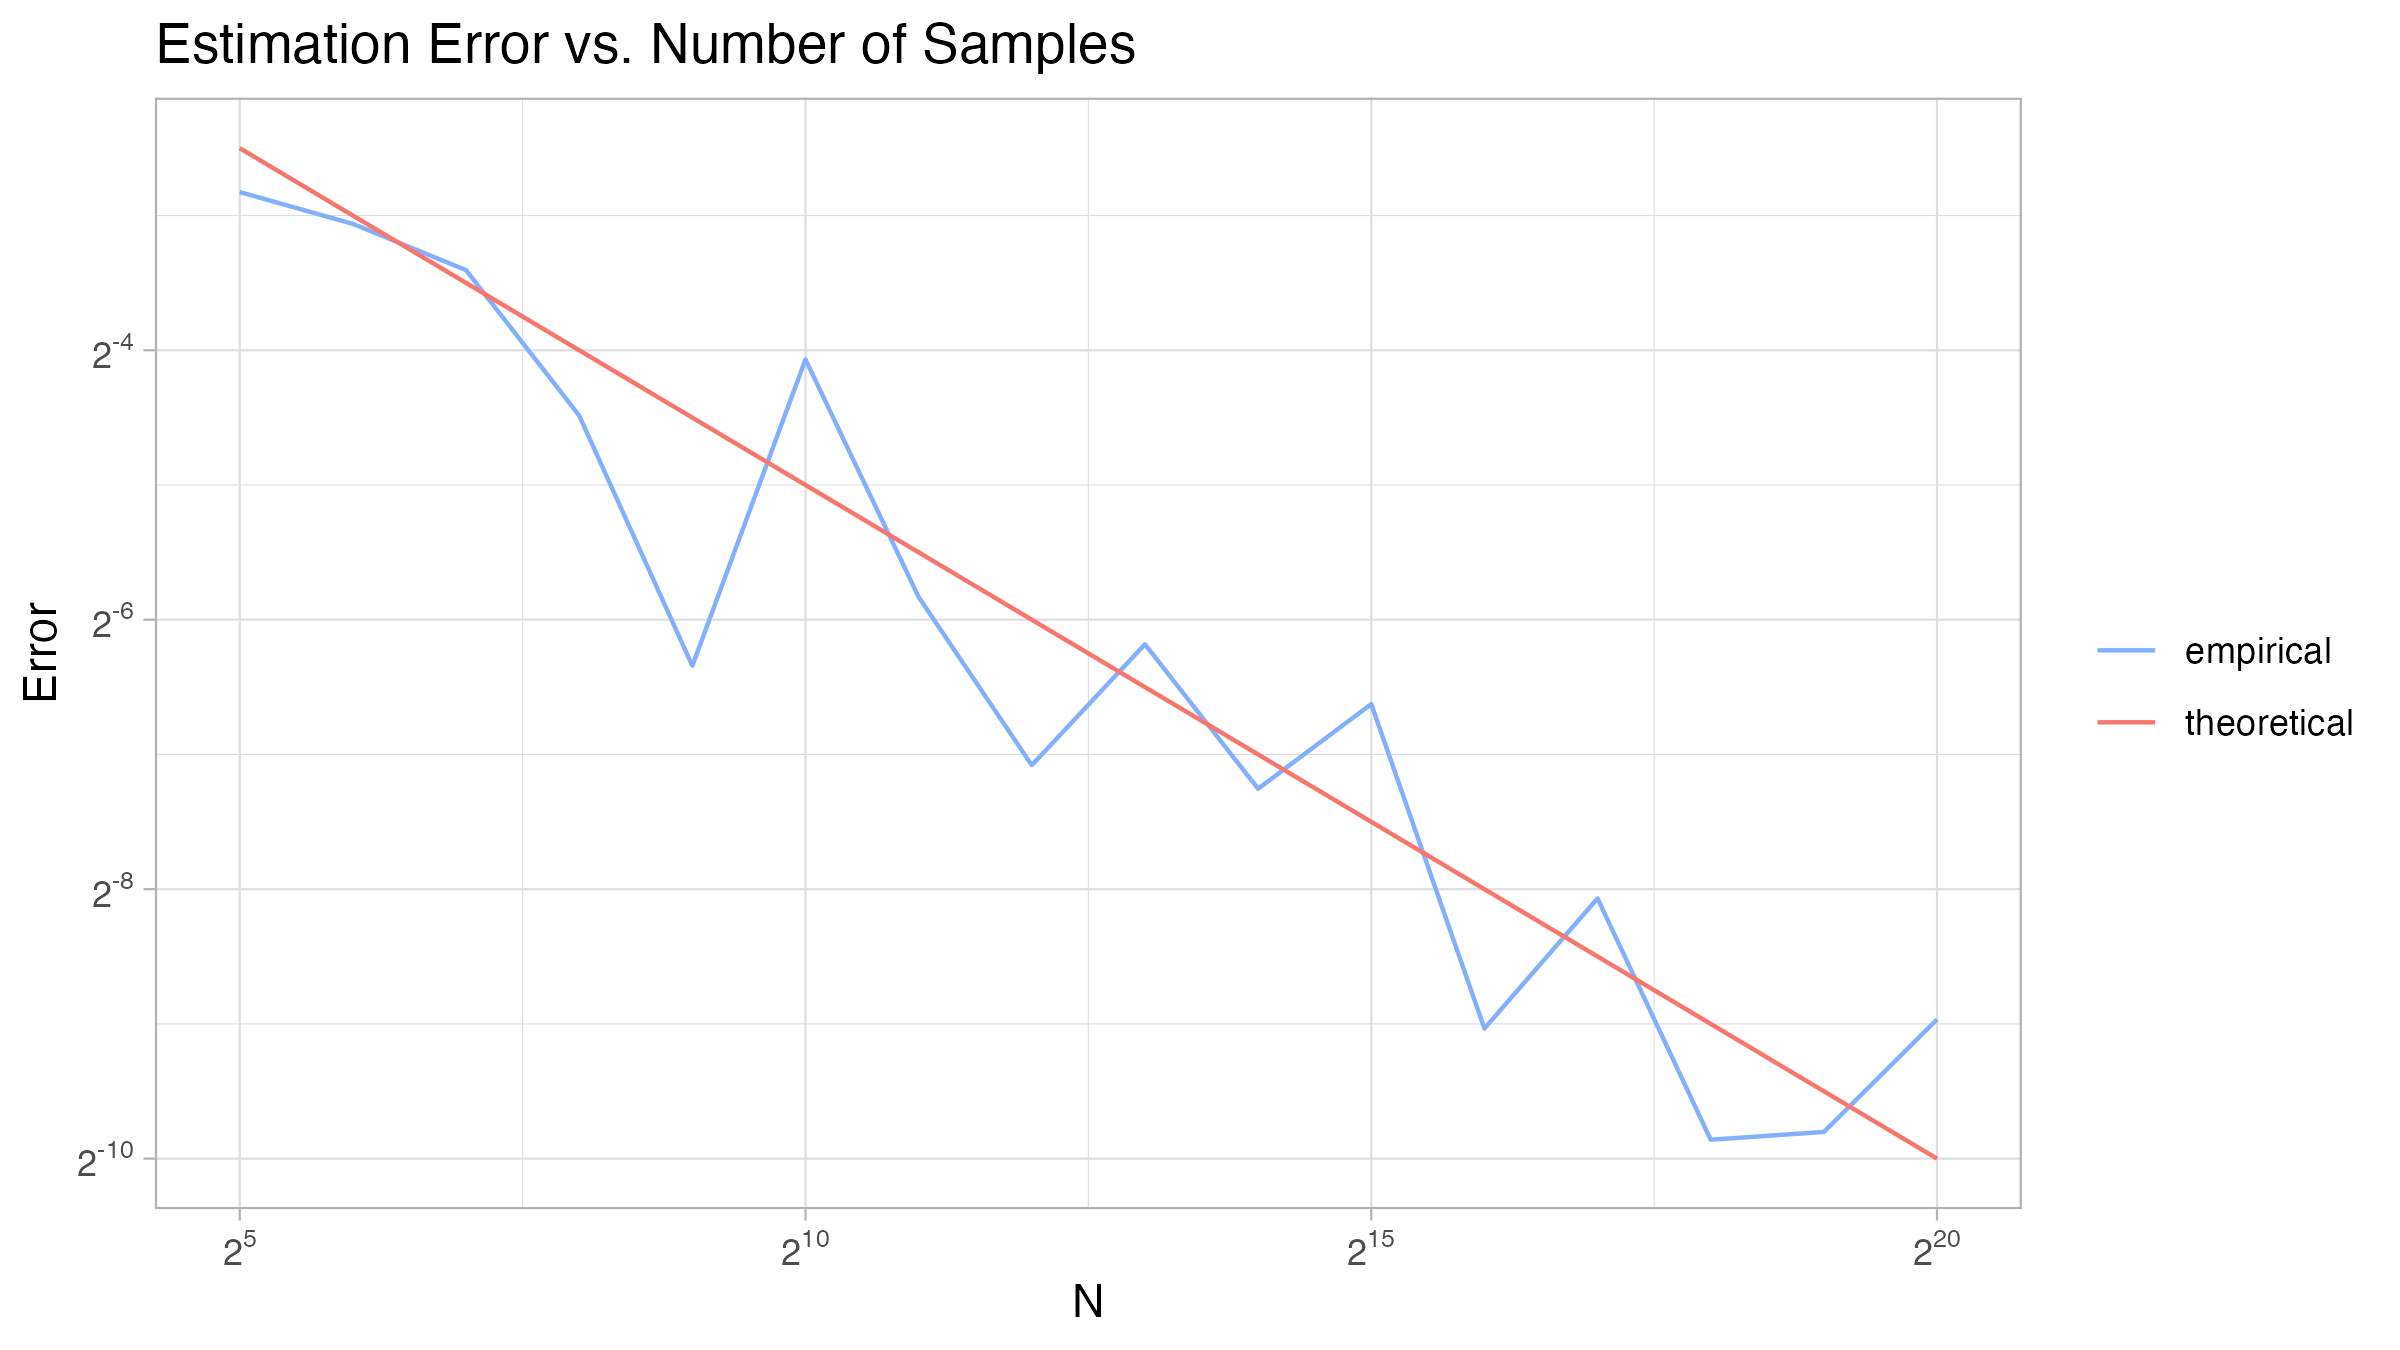
\includegraphics[width=.8\linewidth]{figures/mc-integration2.png}
    \caption{Estimation error for Monte Carlo approximation of $\int_0^{\pi} \sin(x)\,dx$ demonstrating the $\mathcal{O}(n^{-1/2})$ convergence rate. Generated using \href{https://github.com/NikoGerman/Seminar/blob/main/Notebooks/mc-integration.Rmd}{\texttt{mc-integration.Rmd}}.}
    \label{fig:mc-integration2}
\end{figure}


\paragraph{Confidence Intervals}
The asymptotic normality result from Theorem \ref{theorem-clt} enables the construction of confidence intervals for Monte Carlo estimates. 

Since $(\hat{\mu}_n - \mu) \xrightarrow{d} \frac{1}{\sqrt{n}}\mathcal{N}(0, \sigma^2)$, we can approximate the distribution of $\hat{\mu}_n$ as $\mathcal{N}(\mu, \sigma^2/n)$ for large $n$. In practice, the unknown variance $\sigma^2$ is estimated by the sample variance:
\begin{equation}
\hat{\sigma}^2_n = \frac{1}{n-1}\sum_{i=1}^n(\varphi(X_i) - \hat{\mu}_n)^2
\end{equation}
An approximate $(1-\alpha)$-confidence interval for $\mu$ is then given by:
\begin{equation}
\hat{\mu}_n \pm z_{\alpha/2} \frac{\hat{\sigma}_n}{\sqrt{n}}
\end{equation}
where $z_{\alpha/2}$ is the $(1-\alpha/2)$-quantile of the standard normal distribution. This interval provides a measure of uncertainty in the Monte Carlo estimate, with the width decreasing proportionally to $n^{-1/2}$ as the sample size increases.

\section{Sampling from Known Distributions}
\label{sampling}
In the previous chapter, we demonstrated how Monte Carlo methods estimate values that would otherwise be difficult to compute directly. The effectiveness of these methods fundamentally depends on our ability to generate random samples from specified probability distributions.

This chapter introduces various techniques for sampling from known target distributions $f(x)$. We assume access to a pseudo-random number generator (RNG)\footnote{For details on RNGs, see Appendix \ref{appendix:rng}.} that produces samples from the continuous uniform distribution $\text{Unif}(0,1)$. Extensions to sampling from unknown distributions are discussed in Chapter \ref{outlook}.

We begin with the inversion method (Section \ref{Inversion Method}), which provides a direct approach when the cumulative distribution function is invertible. Section \ref{box-muller} focuses on generating samples from the Gaussian distribution. Finally, Section \ref{rejection_sampling} introduces techniques for sampling from less tractable distributions through 
rejection sampling methods. 
A variety of other methods are available, including composition, convolution or copula-based methods (see \cite{lemieux_monte_2009}).

\subsection{Inversion Method}
\label{Inversion Method}

The inversion method allows us to sample from any distribution with an invertible cumulative distribution function (CDF). This fundamental technique transforms uniform random variables into samples from the target distribution \citep{murphy_probabilistic_2023, lemieux_monte_2009}.

\begin{theoremrep}[Inverse Transform]
\label{thm:inverse-transform}
Let $U \sim \text{Unif}(0,1)$ and $F$ be an invertible cumulative distribution function. Then $X = F^{-1}(U)$ has distribution function $F$.
\end{theoremrep}

\begin{proof}
For any $x \in \mathbb{R}$:
\begin{align*}
\mathbb{P}(F^{-1}(U) \leq x) 
&= \mathbb{P}(U \leq F(x)) && \text{(applying $F$ to both sides)} \\
&= F(x) && \text{(since $U \sim \text{Unif}(0,1)$)}
\end{align*}
Therefore, $F^{-1}(U)$ has cumulative distribution function $F$. 
\end{proof}

\begin{example}[Exponential Distribution]
\label{ex:exponential-inversion}
To sample from the exponential distribution $\text{Exp}(\lambda)$, we apply the inversion method. The CDF of the exponential distribution is:
$$F(x;\lambda) = 1 - e^{-\lambda x} \quad \text{for } x \geq 0$$

Setting $u = F(x;\lambda)$ and solving for $x$, we obtain the inverse CDF:
$$F^{-1}(u) = -\frac{1}{\lambda}\ln(1-u)$$

Since $U \sim U(0,1)$ implies $1-U \sim U(0,1)$, we can simplify the implementation by using $U$ directly instead of $1-U$.

\begin{algorithm}[H]
\caption{Random Samples from $\text{Exp}(\lambda)$}
\label{algo:exponential-inversion}
\begin{algorithmic}
    \State $U \gets$ \Call{runif\_01}{1} \Comment{Generate uniform random variable}
    \State $X \gets -\frac{1}{\lambda}\ln(U)$ \Comment{Apply inverse transform}
    \State \Return $X$
\end{algorithmic}
\end{algorithm}

\begin{figure}[h]
    \centering
    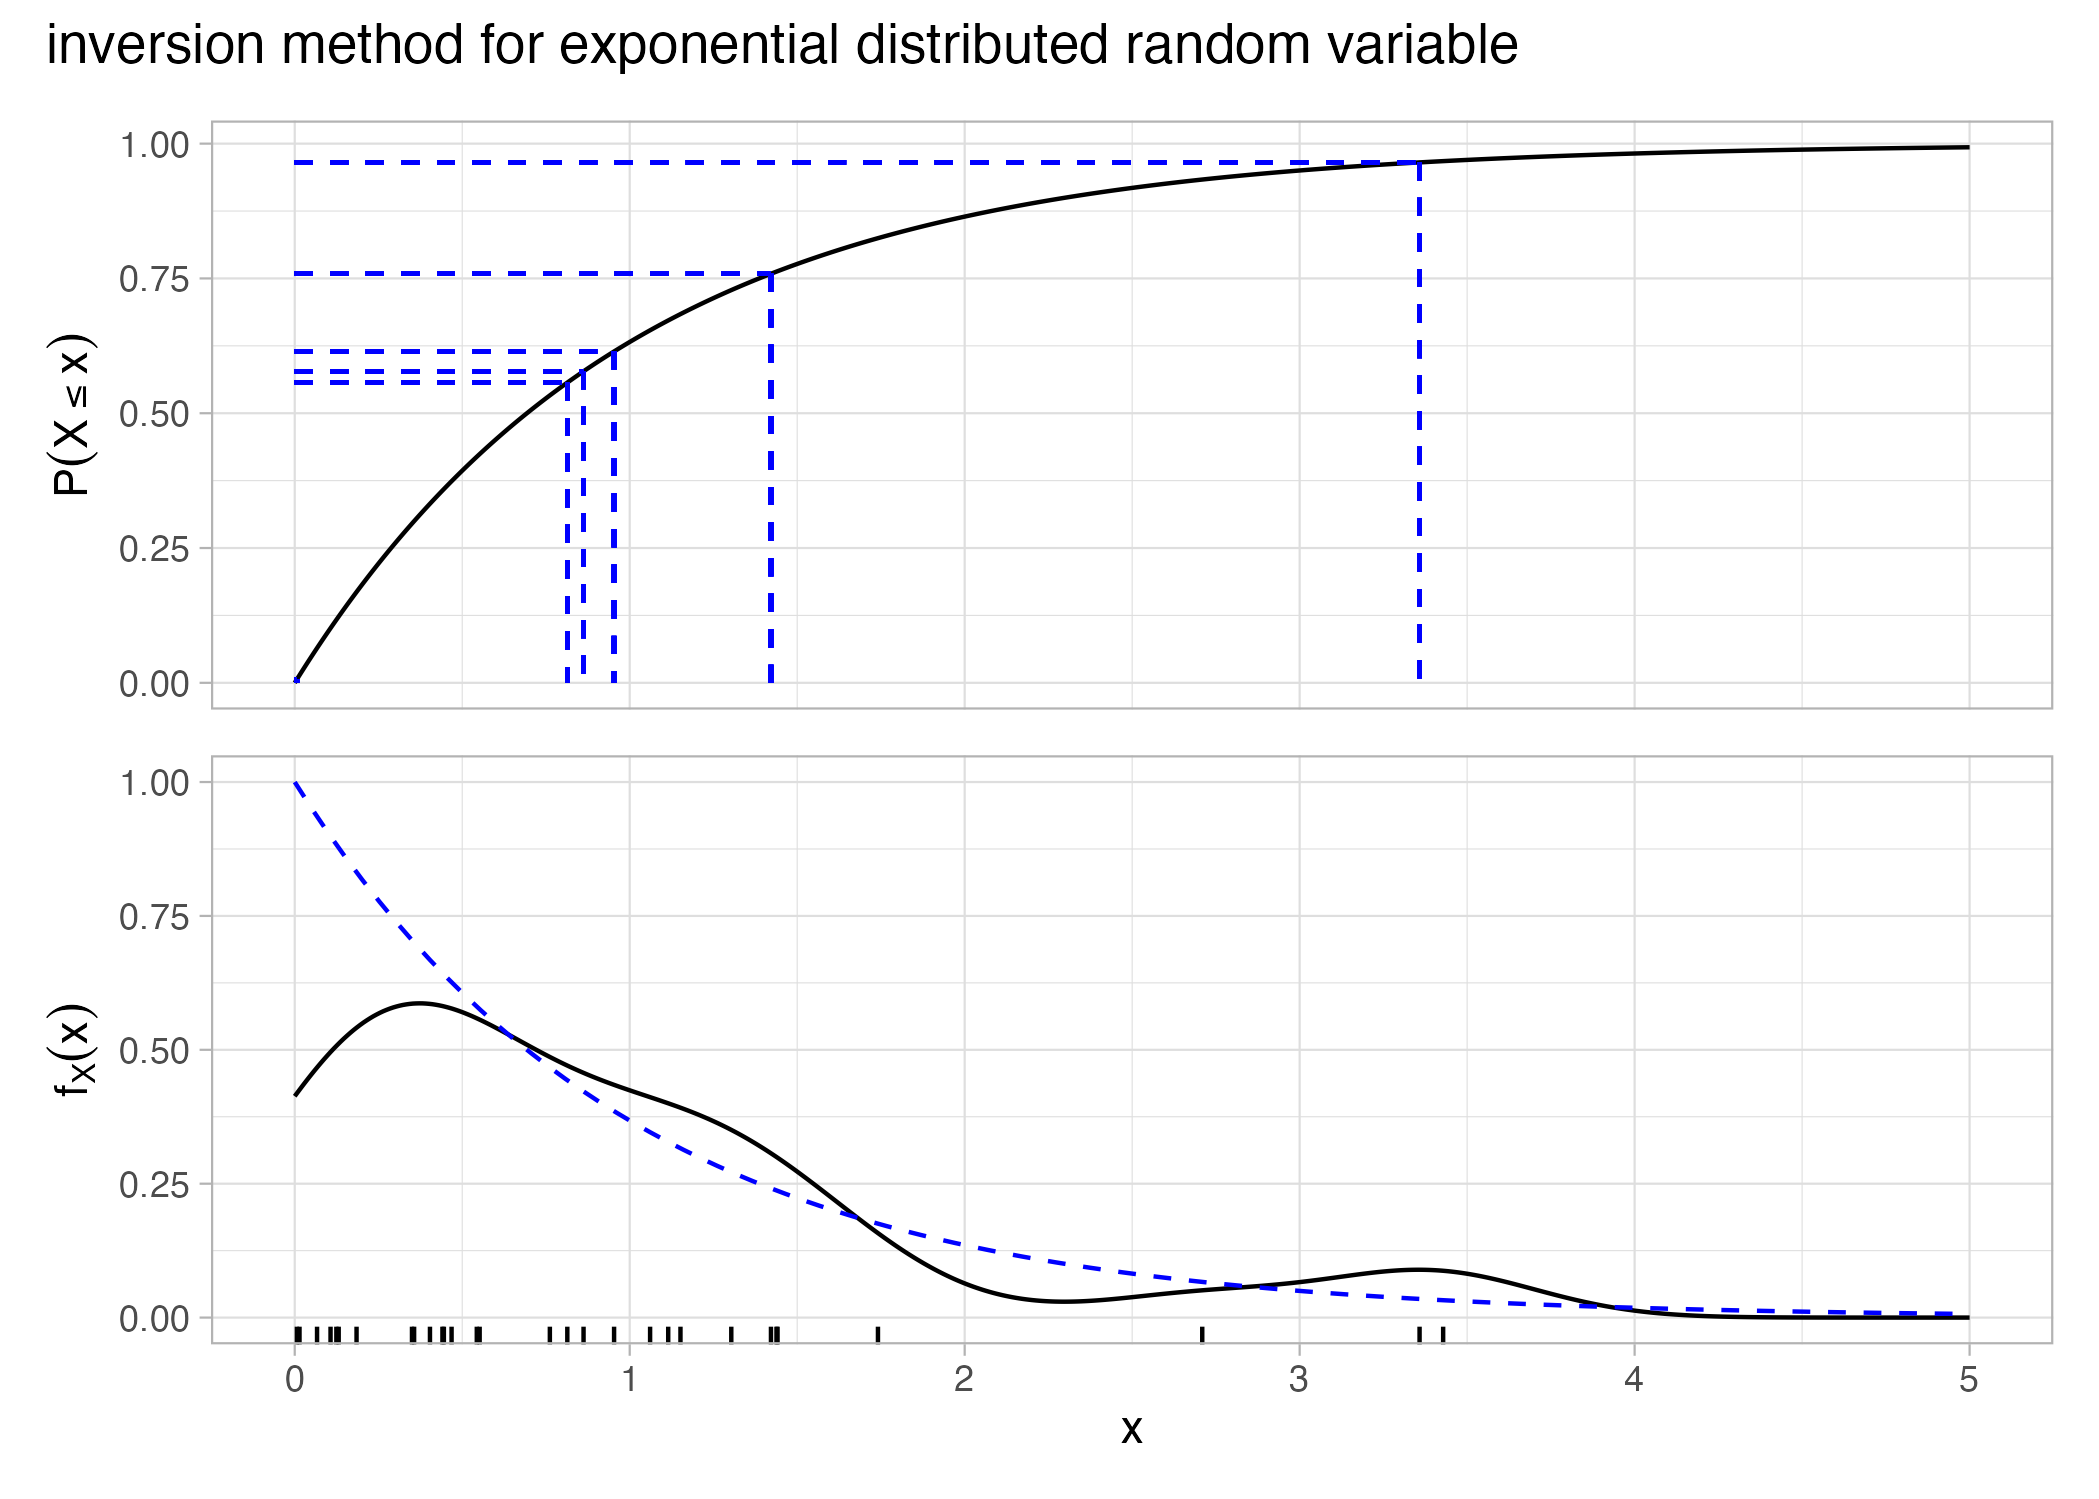
\includegraphics[width=.8\linewidth]{figures/inversion.png}
    \caption{Illustration of the inversion method for generating $\text{Exp}(1)$ random variables. The upper panel demonstrates the transformation process: uniform random samples $U \sim \text{Unif}(0,1)$ are mapped through the inverse cumulative distribution function to yield exponential random variables $X = F^{-1}(U) \sim \text{Exp}(1)$. The lower panel compares the empirical distribution of the generated samples (solid black line) against the theoretical exponential density (dashed blue line), validating the accuracy of the inversion method. Generated using \href{https://github.com/NikoGerman/Seminar/blob/main/Notebooks/inversion-method.Rmd}{\texttt{inversion-method.Rmd}}.}
    \label{fig:inversion-method}
\end{figure}
\end{example}


This demonstrates the power of the inversion method: with a single uniform random variable, we can generate samples from the exponential distribution. Further examples of distributions suitable for the inversion method can be found in \cite{owen_monte_2013}.

\subsection{Box-Muller Method}
\label{box-muller}
The Box-Muller transform is a method for generating pairs of independent standard normal random variables from uniform random variables. The method is based on the polar representation of two independent standard normal variables.

\begin{theoremrep}[Box-Muller Transform]
\label{thm:box-muller}
Let $U_1, U_2 \sim \text{Unif}(0,1)$ be independent uniform random variables. Define:
\begin{equation}
    (X_1, X_2) = \Bigl(\sqrt{-2\ln(U_1)} \cos(2\pi U_2), \sqrt{-2\ln(U_1)} \sin(2\pi U_2)\Bigr)
\end{equation}

Then $X_1, X_2 \sim \mathcal{N}(0,1)$ are independent standard normal random variables.
\end{theoremrep}

\begin{proof}
We prove this by transforming to polar coordinates and applying the change of variables formula.

Let $R = \sqrt{-2\ln(U_1)}$ and $\Theta = 2\pi U_2$. We first determine the joint distribution of $(R, \Theta)$.

\textbf{Step 1: Distribution of $R$.}
Since $U_1 \sim \text{Unif}(0,1)$, we have $-\ln(U_1) \sim \text{Exp}(1)$, which implies $-2\ln(U_1) \sim \text{Exp}(1/2)$. Therefore, $R^2 = -2\ln(U_1) \sim \text{Exp}(1/2)$, making $R$ follow a Rayleigh distribution with parameter 1 (see Appendix \ref{appendix:rayleigh}):
$$f_R(r) = re^{-r^2/2} \quad \text{for } r > 0$$

\textbf{Step 2: Distribution of $\Theta$.}
Since $U_2 \sim \text{Unif}(0,1)$, we have $\Theta = 2\pi U_2 \sim \text{Unif}(0, 2\pi)$ with density:
$$f_\Theta(\theta) = \frac{1}{2\pi} \quad \text{for } \theta \in [0, 2\pi)$$

\textbf{Step 3: Joint distribution of $(R, \Theta)$.}
Since $U_1$ and $U_2$ are independent, $R$ and $\Theta$ are also independent. Therefore:
$$f_{R,\Theta}(r, \theta) = f_R(r) \cdot f_\Theta(\theta) = \frac{r}{2\pi} e^{-r^2/2} \quad \text{for } r > 0, \theta \in [0, 2\pi)$$

\textbf{Step 4: Transformation to Cartesian coordinates.}
The transformation $(X_1, X_2) = (R\cos(\Theta), R\sin(\Theta))$ converts from polar to Cartesian coordinates. The Jacobian matrix is:
$$J = \begin{bmatrix}
\cos(\theta) & -r\sin(\theta) \\
\sin(\theta) & r\cos(\theta)
\end{bmatrix}$$

The determinant is $\det(J) = r\cos^2(\theta) + r\sin^2(\theta) = r$.

\textbf{Step 5: Change of variables.}
Using the change of variables formula (see Appendix \ref{appendix:change_of_vars}), the joint density of $(X_1, X_2)$ is:
\begin{align*}
f_{X_1,X_2}(x_1, x_2) &= f_{R,\Theta}(r, \theta) \cdot \frac{1}{|\det(J)|} \\
&= \frac{r}{2\pi} e^{-r^2/2} \cdot \frac{1}{r} \\
&= \frac{1}{2\pi} e^{-(x_1^2 + x_2^2)/2}
\end{align*}
where we used $r^2 = x_1^2 + x_2^2$.

This joint density factors as:
$$f_{X_1,X_2}(x_1, x_2) = \left(\frac{1}{\sqrt{2\pi}} e^{-x_1^2/2}\right) \cdot \left(\frac{1}{\sqrt{2\pi}} e^{-x_2^2/2}\right)$$

Therefore, $X_1$ and $X_2$ are independent standard normal random variables.
\end{proof}

Algorithm \ref{algo:box-muller} is a simple implementation of the Box-Muller method and produces two independent samples $X_1, X_2 \sim \mathcal{N}(0,1)$, an implementation in \texttt{R} can be found at \href{https://github.com/NikoGerman/Seminar/blob/main/Notebooks/box-muller.Rmd}{\texttt{box-muller.Rmd}}.
\paragraph{Multivariate Normal Random Variables}
To generate multivariate normal random variables, we transform independent standard normal variables using linear transformations.

\begin{theoremrep}[Multivariate Normal Transformation]
\label{thm:multivariate-normal}
Let $Z = (Z_1, \ldots, Z_n)^\top \sim \mathcal{N}_n(\mathbf{0}, I)$ be a vector of i.i.d. standard normal random variables, $\boldsymbol{\mu} = (\mu_1, \ldots, \mu_n)^\top$ be a real-valued mean vector, and $\Sigma \in \mathbb{R}^{n\times n}$ be a symmetric, positive definite covariance matrix. If $L$ is the lower triangular matrix from the Cholesky decomposition\footnote{see Appendix \ref{appendix:Cholesky}.} $\Sigma = LL^\top$, then:
\begin{equation}
    X = \boldsymbol{\mu} + LZ \sim \mathcal{N}_n(\boldsymbol{\mu}, \Sigma)
\end{equation}

\end{theoremrep}

\begin{proof}
We prove this by showing that $X$ has the correct mean and covariance structure.

\textbf{Mean:}
\begin{align*}
\mathbb{E}[X] &= \mathbb{E}[\boldsymbol{\mu} + LZ] \\
&= \mathbb{E}[\boldsymbol{\mu}] + L\mathbb{E}[Z] \\
&= \boldsymbol{\mu} + L \cdot \mathbf{0} = \boldsymbol{\mu}
\end{align*}

\textbf{Covariance:}
\begin{align*}
\text{Cov}(X) &= \text{Cov}(\boldsymbol{\mu} + LZ) \\
&= \text{Cov}(LZ) \\
&= L \cdot \text{Cov}(Z) \cdot L^\top \\
&= L \cdot I_n \cdot L^\top = LL^\top = \Sigma
\end{align*}

Since $X$ is a linear transformation of jointly normal random variables, $X$ is also multivariate normal with mean $\boldsymbol{\mu}$ and covariance $\Sigma$.
\end{proof}

This transformation allows us to generate samples from any multivariate normal distribution using only independent standard normal samples (see Figure \ref{fig:multivariate_normal}).

\begin{figure}[h]
    \centering
    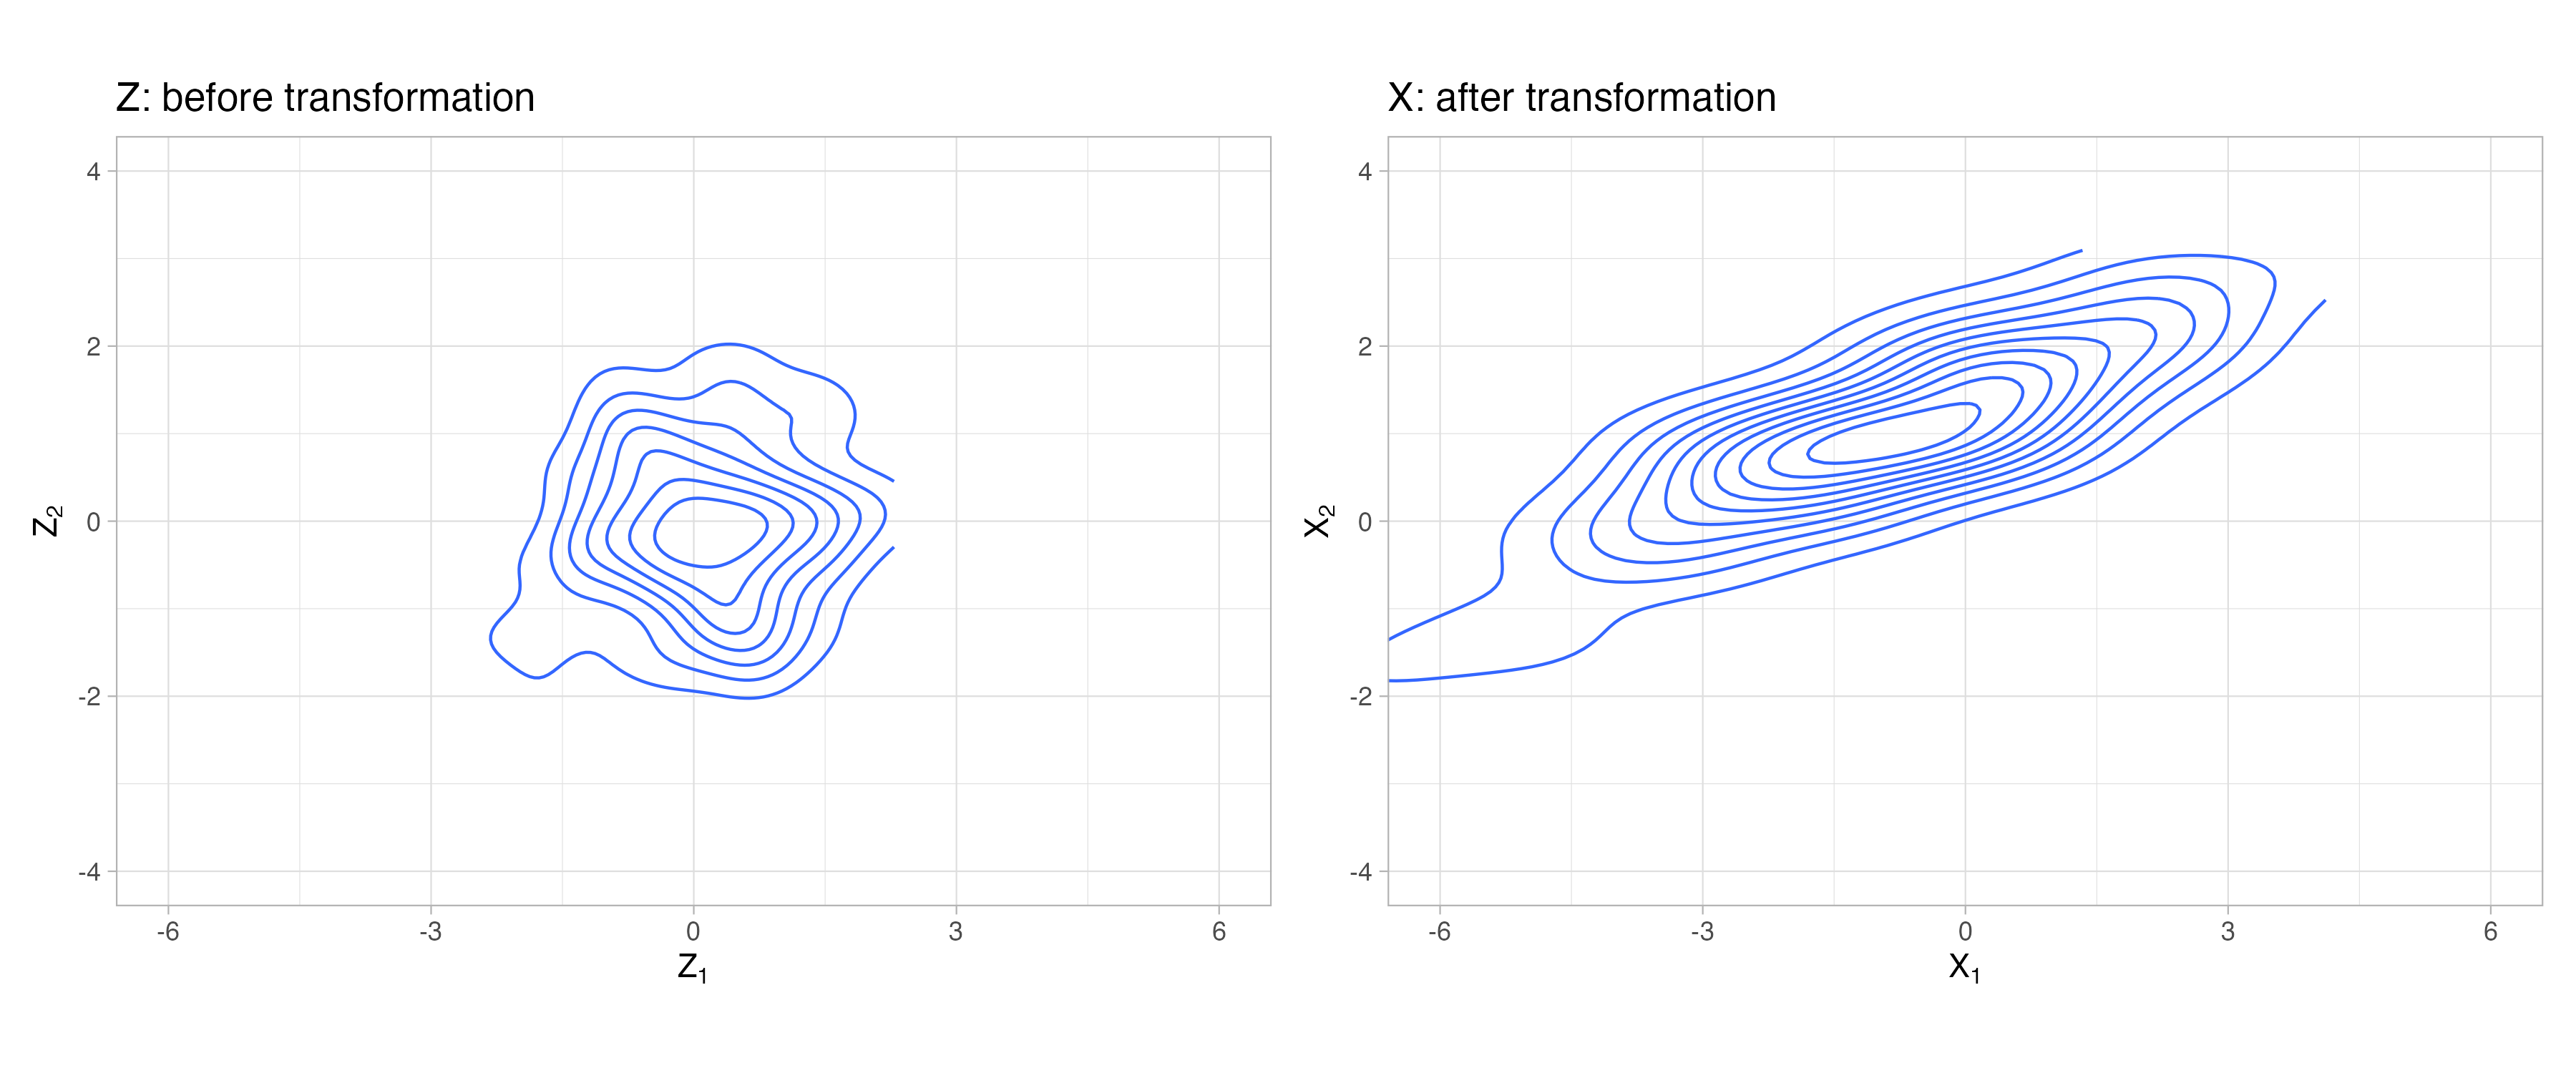
\includegraphics[width=.8\linewidth]{figures/bivariate.png}
    \caption{Visualization of the transformation from standard bivariate normal $\mathcal{N}_2(\boldsymbol{0}, I)$ (left panel) to general bivariate normal $\mathcal{N}_2(\boldsymbol{\mu}, \Sigma)$ (right panel) distributions. The contour plots illustrate the geometric effect of this transformation on the distribution's shape and location. Generated using \href{https://github.com/NikoGerman/Seminar/blob/main/Notebooks/bivariate-normal.Rmd}{\texttt{bivariate-normal.Rmd}}.}
    \label{fig:multivariate_normal}
\end{figure}

\subsection{Acceptance-Rejection}
\label{rejection_sampling}

When the target distribution with density $p(x)$ from which we want to sample is intractable for direct sampling methods (yet somehow easy to evaluate), the \textit{acceptance-rejection} algorithm provides an alternative approach. The idea is to sample from an envelope distribution and then accept or reject these samples according to some criterion. Although this approach wastes some computational effort by throwing away samples, it provides a powerful way to generate samples from complex distributions.

\subsubsection{Basic Rejection Sampling}
Instead of sampling directly from $f(x)$, we sample from $r(x)$, where $r(x)$ is a probability density function and the following envelope condition is satisfied:
\begin{equation*}
    T \cdot r(x) \geq f(x) \quad \forall x
\end{equation*}

We define $t(x) = T \cdot r(x)$. The function $t(x)$ need not be normalized, but must satisfy the condition $T = \int t(x)dx < \infty$.

The acceptance-rejection algorithm can be characterized as follows:
\begin{enumerate}
    \item Generate a candidate $\tilde{X} \sim r$
    \item Generate $U \sim \text{Unif}(0,1)$ independent of $\tilde{X}$
    \item If $U \leq \frac{f(\tilde{X})}{t(\tilde{X})}$, accept and set $X = \tilde{X}$; otherwise, reject and return to step 1.
\end{enumerate}

\begin{theoremrep}[Acceptance-Rejection Sampling]
Let $X$ denote an accepted sample. Then $X$ has cumulative distribution function $F(x) = \int_{-\infty}^x f(y)dy$.
\end{theoremrep}

\begin{proof}
We need to show that 
$$\mathbb{P}(X \leq x) = \mathbb{P}\left(\tilde{X} \leq x \mid U \leq \frac{f(\tilde{X})}{t(\tilde{X})}\right) = F(x)$$

Using the definition of conditional probability:
\begin{align*}
    \mathbb{P}\left(\tilde{X} \leq x \mid U \leq \frac{f(\tilde{X})}{t(\tilde{X})}\right) &= \frac{
    \mathbb{P}\left(\tilde{X} \leq x, U \leq \frac{f(\tilde{X})}{t(\tilde{X})}\right)}{\mathbb{P}\left(U \leq \frac{f(\tilde{X})}{t(\tilde{X})}\right)}
\end{align*}

For the numerator, using the law of total probability and independence of $U$ and $\tilde{X}$:
\begin{align*}
    \mathbb{P}\left(\tilde{X} \leq x, U \leq \frac{f(\tilde{X})}{t(\tilde{X})}\right) &= \int_{-\infty}^x \mathbb{P}\left(U \leq \frac{f(y)}{t(y)}\right) r(y) dy \\
    &= \int_{-\infty}^x \frac{f(y)}{t(y)} r(y) dy \\
    &= \frac{1}{T}\int_{-\infty}^x f(y) dy
\end{align*}

For the denominator:
\begin{align*}
    \mathbb{P}\left(U \leq \frac{f(\tilde{X})}{t(\tilde{X})}\right) &= \int_{-\infty}^{\infty} \frac{f(y)}{t(y)} r(y) dy \\
    &= \frac{1}{T}\int_{-\infty}^{\infty} f(y) dy = \frac{1}{T}
\end{align*}

Therefore:
\begin{align*}
    \mathbb{P}\left(\tilde{X} \leq x \mid U \leq \frac{f(\tilde{X})}{t(\tilde{X})}\right) &= \frac{\frac{1}{T}\int_{-\infty}^x f(y) dy}{\frac{1}{T}} = \int_{-\infty}^x f(y) dy = F(x)
\end{align*}
\end{proof}

The implementation of acceptance-rejection is straight-forward (see Algorithm \ref{algo:acceptance-rejection}). The main challenge is sampling from $r(x)$ and possibly the evaluation of $f(\cdot)$ and $t(\cdot)$. For the former challenge we assume to have access to some algorithm \texttt{rand\_r()}, which samples from $r(x)$.

\subsubsection{Adaptive Rejection Sampling}
Adaptive rejection sampling is an extension of the basic acceptance-rejection method that automatically constructs and refines the envelope function during the sampling process. For log-concave target densities, the algorithm exploits the property that tangent lines to the log-density provide a tight upper bound. The method begins with an initial set of tangent points and iteratively improves the piecewise-linear envelope by adding new tangent lines at rejected sample locations. Algorithm \ref{algo:adaptive-rejection} demonstrates a basic implementation. 

The adaptive refinement ensures that the envelope becomes increasingly efficient over time, dramatically reducing the rejection rate as more samples are drawn. For more detailed information on adaptive rejection sampling, see \cite{murphy_probabilistic_2023}.


\section{Variance Reduction Techniques}
\label{variance-control}
Variance reduction techniques aim to improve Monte Carlo integration by finding alternative functions whose integrals equal the original but have smaller variance. The goal is to achieve a reduction in variance while restricting the computational increase\footnote{A measure of the quality of estimators that considers both variance and computation time, is called \textit{Efficiency}. \cite{lemieux_monte_2009}}. We will focus on three methods: In section \ref{importance_sampling} we will discuss \textit{Importance Sampling}, likely the most well-known technique. We then follow up in section \ref{control_variates} with a technique called \textit{Control Variates} and will finish in section \ref{Rao-B} with \textit{Conditional Monte Carlo}. There are many more techniques\footnote{for example \textit{Antithetic Sampling} and \textit{Common Random Numbers}, for further information see \cite{murphy_probabilistic_2023, lemieux_monte_2009}.} in existence, and \cite{lemieux_monte_2009} even mentions the possibility to combine them.

\subsection{Importance Sampling}
\label{importance_sampling}

Importance sampling directs sampling effort toward the most important regions of the integration domain, making it particularly useful for rare event simulation. Instead of sampling from the original density $f(x)$, we sample from an alternative density $g(x)$ and correct using likelihood ratios. We will focus on two fundamental variants: \textit{Direct Importance Sampling and Self-Normalized Importance Sampling}, as discussed in \cite{lemieux_monte_2009}. 

Although other variants exist, such as \textit{Annealed importance sampling} (discussed in \cite{murphy_probabilistic_2023}), they fall outside the scope of this paper.

\subsubsection{Direct Importance Sampling}

The standard importance sampling estimator transforms $\mu = \int \varphi(x)f(x)dx$ into:
\begin{equation}
\hat{\mu}_{is} = \frac{1}{n}\sum_{i=1}^n \varphi(\tilde{x}_i)L(\tilde{x}_i)
\end{equation}
where $L(x) = f(x)/g(x)$ is the likelihood ratio and $\tilde{x}_i \sim g(x)$. 

\begin{theoremrep}[Unbiasedness of Importance Sampling]
The importance sampling estimator $\hat{\mu}_{is}$ is unbiased for $\mu$.
\end{theoremrep}

\begin{proof}
We compute the expectation:
\begin{align*}
E(\hat{\mu}_{is}) &= E\left[\frac{1}{n}\sum_{i=1}^n \varphi(\tilde{X}_i)L(\tilde{X}_i)\right]\\
&= E[\varphi(\tilde{X})L(\tilde{X})]\\
&= \int \varphi(x)L(x)g(x)dx\\
&= \int \varphi(x)\frac{f(x)}{g(x)}g(x)dx\\
&= \int \varphi(x)f(x)dx = \mu
\end{align*}
\end{proof}

\begin{theoremrep}[Variance of Importance Sampling]
The variance of the importance sampling estimator is:
\begin{equation}
\text{Var}[\hat{\mu}_{is}] = \frac{1}{n}\left(E_f[\varphi^2(X)L(X)] - \mu^2\right)
\end{equation}
\end{theoremrep}

\begin{proof}
Let $\tilde{X}_1, \ldots, \tilde{X}_n$ be independent samples from $g(x)$. We assume that $g(x) > 0$ whenever $\varphi(x)f(x) \neq 0$ to ensure the likelihood ratio is well-defined.

\textbf{Step 1: Variance Decomposition}
By the independence of the samples $\tilde{X}_i$, the variance of the estimator is:
\begin{align*}
\text{Var}[\hat{\mu}_{is}] &= \text{Var}\left[\frac{1}{n}\sum_{i=1}^n \varphi(\tilde{X}_i)L(\tilde{X}_i)\right]\\
&= \frac{1}{n^2}\sum_{i=1}^n \text{Var}[\varphi(\tilde{X}_i)L(\tilde{X}_i)]\\
&= \frac{1}{n}\text{Var}[\varphi(\tilde{X})L(\tilde{X})]
\end{align*}

\textbf{Step 2: Variance Formula}
Using the standard variance identity $\text{Var}[Y] = E[Y^2] - E[Y]^2$, we have:
\begin{align*}
\text{Var}[\varphi(\tilde{X})L(\tilde{X})] &= E[(\varphi(\tilde{X})L(\tilde{X}))^2] - (E[\varphi(\tilde{X})L(\tilde{X})])^2\\
&= E[\varphi^2(\tilde{X})L^2(\tilde{X})] - \mu^2
\end{align*}
where we used the unbiasedness property $E[\varphi(\tilde{X})L(\tilde{X})] = \mu$.

\textbf{Step 3: Rewriting as Expectation Under Original Distribution}
We can rewrite the Expectation by factoring out one $f(x)$ term:
\begin{align*}
E[\varphi^2(\tilde{X})L^2(\tilde{X})] 
&= \int_{-\infty}^{\infty} \varphi^2(x)L^2(x) \cdot g(x) \, dx \\
&= \int_{-\infty}^{\infty} \varphi^2(x)\frac{f^2(x)}{g^2(x)} \cdot g(x) \, dx\\
&= \int_{-\infty}^{\infty} \varphi^2(x)\frac{f(x)}{g(x)} \cdot f(x) \, dx\\
&= \int_{-\infty}^{\infty} \varphi^2(x)L(x) \cdot f(x) \, dx\\
&= E_f[\varphi^2(X)L(X)]
\end{align*}
where $E_f[\cdot]$ denotes expectation with respect to the original density $f(x)$.

\textbf{Step 4: Final Result}
Combining the steps above, we obtain:
\begin{align*}
\text{Var}[\hat{\mu}_{is}] &= \frac{1}{n}\text{Var}[\varphi(\tilde{X})L(\tilde{X})]\\
&= \frac{1}{n}\left(E[\varphi^2(\tilde{X})L^2(\tilde{X})] - \mu^2\right)\\
&= \frac{1}{n}\left(E_f[\varphi^2(X)L(X)] - \mu^2\right)
\end{align*}
\end{proof}

This shows that the variance of the importance sampling estimator depends on $E_f[\varphi^2(X)L(X)]$ under the original distribution $f(x)$. Variance reduction occurs when $E_f[\varphi^2(X)L(X)] \leq E_f[\varphi^2(X)]$. Under certain conditions, there exists an optimal choice for $g(x)$ (see \cite{lemieux_monte_2009}).

\begin{theoremrep}[Optimal Importance Distribution]
Suppose $\mu = \int \varphi(x)f(x)dx \neq 0$ is known. Then the optimal importance distribution that minimizes the variance is:
\begin{equation}
    g^*(x) = \frac{\varphi(x)f(x)}{\mu}
\end{equation}
and this choice yields zero variance for the importance sampling estimator.
\end{theoremrep}

\begin{proof}
First, we verify that $g^*(x)$ is a valid probability density function. We have:
$$\int_{-\infty}^{\infty} g^*(x) dx = \int_{-\infty}^{\infty} \frac{\varphi(x)f(x)}{\mu} dx = \frac{1}{\mu} \int_{-\infty}^{\infty} \varphi(x)f(x) dx = \frac{\mu}{\mu} = 1$$

The likelihood ratio is:
$$L^*(x) = \frac{f(x)}{g^*(x)} = \frac{f(x)}{\frac{\varphi(x)f(x)}{\mu}} = \frac{\mu}{\varphi(x)}$$
where we assume $\varphi(x) \neq 0$ on the relevant support.

Now we calculate $E_f[\varphi^2(X)L^*(X)]$:
\begin{align*}
    E_f[\varphi^2(X)L^*(X)] 
    &= E_f \left[ \varphi^2(X) \cdot \frac{\mu}{\varphi(X)} \right] \\
    &= \mu \cdot E_f[\varphi(X)] \\
    &= \mu \cdot \mu = \mu^2
\end{align*}

Applying the variance formula for importance sampling:
\begin{align*}
    \text{Var}[\hat{\mu}_{is}] 
    &= \frac{1}{n}\left(E_f[\varphi^2(X)L^*(X)] - \mu^2\right) \\
    &= \frac{1}{n} \left(\mu^2 - \mu^2\right) \\
    &= 0
\end{align*}

Thus, the optimal importance distribution $g^*(x)$ achieves zero variance.
\end{proof}

While this result is primarily theoretical—since knowing $\mu$ exactly would make estimation unnecessary—it provides valuable guidance for choosing effective importance distributions in practice. The optimal form $g^*(x) \propto \varphi(x)f(x)$ suggests that the importance distribution should concentrate sampling effort in regions where the integrand $\varphi(x)f(x)$ is large. In practical applications, one can approximate this optimal distribution by choosing $g(x)$ to be roughly proportional to $\varphi(x)f(x)$ or to mimic its shape, thereby achieving substantial variance reduction even when the exact optimal distribution is unknown.



\subsubsection{Self-normalized Importance Sampling}

The self-normalized or \textit{weighted} importance sampling estimator has the following form:
\begin{equation}
\hat{\mu}_{is,w} = \sum_{i=1}^n w_i\varphi(\tilde{x}_i) 
\end{equation}

and uses normalized likelihood ratios as weights:

\begin{equation*}
w_i = \frac{L(\tilde{x}_i)}{\sum_{i=1}^n L(\tilde{x}_i)}
\end{equation*}

It is easy to see, that the weights are bounded: $w_i \in [0, 1] \quad \forall \quad i=1,...,n$. Additionally, the weights add up to 1. This approach can handle complicated densities with unknown normalizing constants, and is biased, yet consistent\footnote{An estimator $\hat{\mu}$ is called \textit{consistent} if $Bias(\hat{\mu}) \to 0$ for $n \to \infty$} (see \cite{lemieux_monte_2009, murphy_probabilistic_2023}). The normalization cancels unknown constants in both $f$ and $g$.

\subsection{Control Variates}
\label{control_variates}

Control variates reduce variance by exploiting correlation with auxiliary variables whose expectations are known. The control variate method introduces a baseline function $\beta(X)$ with known expectation $E[\beta(X)] = \mu_\beta$. The control variate estimator is:
\begin{equation}
\hat{\mu}_{cv} = \frac{1}{n}\sum_{i=1}^n [\varphi(X_i) + c(\mu_\beta - \beta(X_i))]
\end{equation}
where $c$ is a coefficient to be determined optimally.

\begin{theoremrep}[Unbiasedness of Control Variates]
The control variate estimator $\hat{\mu}_{cv}$ is unbiased for any choice of coefficient $c$.
\end{theoremrep}

\begin{proof}
\begin{align*}
E[\hat{\mu}_{cv}] &= E\left[\frac{1}{n}\sum_{i=1}^n [\varphi(X_i) + c(\mu_\beta - \beta(X_i))]\right]\\
&= E[\varphi(X)] + c(E[\mu_\beta] - E[\beta(X)])\\
&= E[\varphi(X)] + c(\mu_\beta - \mu_\beta) = \mu
\end{align*}
\end{proof}

\begin{theoremrep}[Variance of Control Variate Estimator]
The variance of the control variate estimator is:
\begin{equation}
\text{Var}(\hat{\mu}_{cv}) = \frac{1}{n}[\text{Var}(\varphi(X)) + c^2\text{Var}(\beta(X)) - 2c\text{Cov}(\varphi(X), \beta(X))]
\end{equation}
\end{theoremrep}

\begin{proof}
\begin{align*}
\text{Var}(\hat{\mu}_{cv}) &= \text{Var}\left(\frac{1}{n}\sum_{i=1}^n [\varphi(X_i) + c(\mu_\beta - \beta(X_i))]\right)\\
&= \frac{1}{n}\text{Var}(\varphi(X) + c(\mu_\beta - \beta(X)))\\
&= \frac{1}{n}\text{Var}(\varphi(X) - c\beta(X))\\
&= \frac{1}{n}[\text{Var}(\varphi(X)) + c^2\text{Var}(\beta(X)) - 2c\text{Cov}(\varphi(X), \beta(X))]
\end{align*}
\end{proof}

\begin{theoremrep}[Optimal Control Variate Coefficient]
The optimal coefficient that minimizes the variance of $\hat{\mu}_{cv}$ is:
\begin{equation}
c^* = \frac{\text{Cov}(\varphi(X), \beta(X))}{\text{Var}(\beta(X))}
\end{equation}
and the resulting optimal variance is:
\begin{equation}
\text{Var}(\hat{\mu}_{cv}) = (1 - \rho_{\varphi,\beta}^2)\text{Var}(\hat{\mu}) \leq \text{Var}(\hat{\mu})
\end{equation}
where $\rho_{\varphi,\beta}^2$ is the squared correlation between $\varphi(X)$ and $\beta(X)$.
\end{theoremrep}

\begin{proof}
To minimize the variance, we take the derivative with respect to $c$ and set it to zero:
\begin{align*}
\frac{\partial}{\partial c}\text{Var}(\hat{\mu}_{cv}) &= \frac{1}{n}[2c\text{Var}(\beta(X)) - 2\text{Cov}(\varphi(X), \beta(X))] = 0
\end{align*}

Solving for $c$ yields:
$$c^* = \frac{\text{Cov}(\varphi(X), \beta(X))}{\text{Var}(\beta(X))}$$

Substituting $c^*$ into the variance expression:
\begin{align*}
\text{Var}(\hat{\mu}_{cv}) &= \frac{1}{n}\left[\text{Var}(\varphi(X)) - \frac{[\text{Cov}(\varphi(X), \beta(X))]^2}{\text{Var}(\beta(X))}\right]\\
&= \frac{1}{n}\text{Var}(\varphi(X))\left[1 - \frac{[\text{Cov}(\varphi(X), \beta(X))]^2}{\text{Var}(\varphi(X))\text{Var}(\beta(X))}\right]\\
&= (1 - \rho_{\varphi,\beta}^2)\text{Var}(\hat{\mu})
\end{align*}
\end{proof}

High correlation between $\varphi(X)$ and $\beta(X)$ maximizes variance reduction, as seen in the $(1 - \rho_{\varphi,\beta}^2)$ factor. For further information, see \cite{murphy_probabilistic_2023, lemieux_monte_2009}.

\subsection{Conditional Monte Carlo}
\label{Rao-B}

Conditional Monte Carlo reduces variance by analytically marginalizing out some variables instead of sampling them. Consider estimating $\mu = E[\varphi(X,Y)]$ where the conditional expectation $E[\varphi(X,Y)|X]$ can be computed tractably.

The standard Monte Carlo estimator uses samples $(X_s, Y_s) \sim f(X,Y)$:
\begin{equation}
\hat{\mu}_{MC} = \frac{1}{n}\sum_{s=1}^n \varphi(X_s, Y_s)
\end{equation}

The conditional Monte Carlo estimator samples only $X_s \sim f(X)$ and computes:
\begin{equation}
\hat{\mu}_{CMC} = \frac{1}{n}\sum_{s=1}^n E[\varphi(X,Y)|X_s]
\end{equation}

\begin{theoremrep}[Unbiasedness of Conditional Monte Carlo]
The conditional Monte Carlo estimator $\hat{\mu}_{CMC}$ is unbiased for $\mu$.
\end{theoremrep}

\begin{proof}
\begin{align*}
E[\hat{\mu}_{CMC}] &= E\left[\frac{1}{n}\sum_{s=1}^n E[\varphi(X,Y)|X_s]\right]\\
&= E[E[\varphi(X,Y)|X]]\\
&= E[\varphi(X,Y)] \quad \text{(by the law of total expectation)}\\
&= \mu
\end{align*}
\end{proof}

\begin{theoremrep}[Variance Reduction of Conditional Monte Carlo]
The conditional Monte Carlo estimator has variance:
\begin{equation}
\text{Var}(\hat{\mu}_{CMC}) = \frac{1}{n}\text{Var}(E[\varphi(X,Y)|X]) \leq \frac{1}{n}\text{Var}(\varphi(X,Y)) = \text{Var}(\hat{\mu}_{MC})
\end{equation}
with equality if and only if $\varphi(X,Y)$ is completely determined by $X$.
\end{theoremrep}

\begin{proof}
The variance of the conditional Monte Carlo estimator is:
\begin{align*}
\text{Var}(\hat{\mu}_{CMC}) &= \text{Var}\left(\frac{1}{n}\sum_{s=1}^n E[\varphi(X,Y)|X_s]\right)\\
&= \frac{1}{n}\text{Var}(E[\varphi(X,Y)|X])
\end{align*}

By the law of total variance:
\begin{align*}
\text{Var}(\varphi(X,Y)) &= \text{Var}(E[\varphi(X,Y)|X]) + E[\text{Var}(\varphi(X,Y)|X)]
\end{align*}

Rearranging gives us:
\begin{align*}
\text{Var}(E[\varphi(X,Y)|X]) &= \underbrace{\text{Var}(\varphi(X,Y))}_{\text{Variance of Naive Monte Carlo estimator}} - 
\underbrace{E[\text{Var}(\varphi(X,Y)|X)]}_{\geq 0} 
\end{align*}

Therefore:
\begin{align*}
\text{Var}(E[\varphi(X,Y)|X]) &\leq \text{Var}(\varphi(X,Y))
\end{align*}

This gives us:
\begin{align*}
\text{Var}(\hat{\mu}_{CMC}) &= \frac{1}{n}\text{Var}(E[\varphi(X,Y)|X]) \leq \frac{1}{n}\text{Var}(\varphi(X,Y)) = \text{Var}(\hat{\mu}_{MC})
\end{align*}

Equality holds if and only if $E[\text{Var}(\varphi(X,Y)|X)] = 0$, which occurs when $\text{Var}(\varphi(X,Y)|X) = 0$. This happens when $\varphi(X,Y)$ is a deterministic function of $X$ alone.
\end{proof}

The intuition is that we eliminate randomness from $Y$ through analytical integration, sampling only in the reduced dimensional space of $X$. The variance reduction equals $E[\text{Var}(\varphi(X,Y)|X)]$. For further information, see \cite{murphy_probabilistic_2023, lemieux_monte_2009}.

\section{Quasi Monte Carlo}
\label{QMC}
\cite{lemieux_monte_2009} provides a useful characterization of Quasi-Monte Carlo sampling methods:
\begin{quote}
Quasi–Monte Carlo sampling methods are typically used to provide approximations
for multivariate integration problems defined over the unit hypercube.
\end{quote}

In Quasi-Monte Carlo (QMC) methods, random sampling is replaced by carefully constructed deterministic sequences.
Rather than sampling randomly from the $d$-dimensional unit hypercube $[0,1]^d$, QMC methods generate \textit{low discrepancy sequences}\footnote{For a more detailed background on low discrepancy sequences, see Appendix \ref{appendix:low_discrepancy}.} for evaluating integrals of the form $\int_{[0,1]^d} f(x) \,dx$. These sequences minimize clustering and gaps, providing more systematic and uniform coverage of the integration domain.
This approach often achieves better convergence rates than standard Monte Carlo methods, particularly for smooth integrands.


\paragraph{Deterministic Nature and Its Implications}
While the systematic point placement of QMC often leads to faster convergence rates, it has two key limitations. First, the Central Limit Theorem does not apply to deterministic sequences, making standard error estimation techniques unusable; concequently QMC does not provide confidence intervals. Second, QMC performance depends heavily on integrand smoothness.

\paragraph{Comparison with Traditional Numerical Integration}
When projected onto lower-dimensional subspaces, grid points of regular grids often collapse onto a much smaller set, creating poor coverage. Low discrepancy sequences are specifically designed to maintain good uniformity properties even under such projections.

A visual comparison can be found in Figure \ref{fig:ex1-samples} (Section \ref{approx-pi}), which illustrates the key differences between these approaches. Random sampling exhibits clustering and gaps, regular grids show systematic coverage but suffer from poor projection properties, while low discrepancy sequences achieve both systematic coverage and retain uniformity under projections.

For a comprehensive treatment of QMC, see \cite{owen_practical_2023}.

\section{Applications}
\label{applications}
\subsection{Approximating $\pi$}
\label{approx-pi}

We demonstrate different sampling strategies through the well-known problem of estimating $\pi$ by approximating the area of a unit circle inscribed in a square. A comprehensive analysis including implementation details and extended theoretical background can be found at \href{https://nikogerman.github.io/Seminar/Notebooks/example1-estimating-pi.html}{\texttt{example1-estimating-pi.html}}. In the following, we discuss only the general setup and key results.

Since the unit circle has area $\pi$ and the enclosing square $[-1,1] \times [-1,1]$ has area 4, we obtain the estimator $\hat{\pi} = 4 \cdot \mathbb{P}(X^2 + Y^2 \leq 1)$ where $(X,Y)$ are sampled from the square.

\textbf{Sampling Methods Compared:} We compare uniform Monte Carlo sampling, importance sampling with $\mathcal{N}(0, \sigma^2 I_2)$ where $\sigma = 1/3$, quasi-Monte Carlo using Sobol sequences, and grid-based deterministic quadrature.

\begin{figure}[h]
    \centering
    \begin{subfigure}[b]{0.48\textwidth}
        \centering
        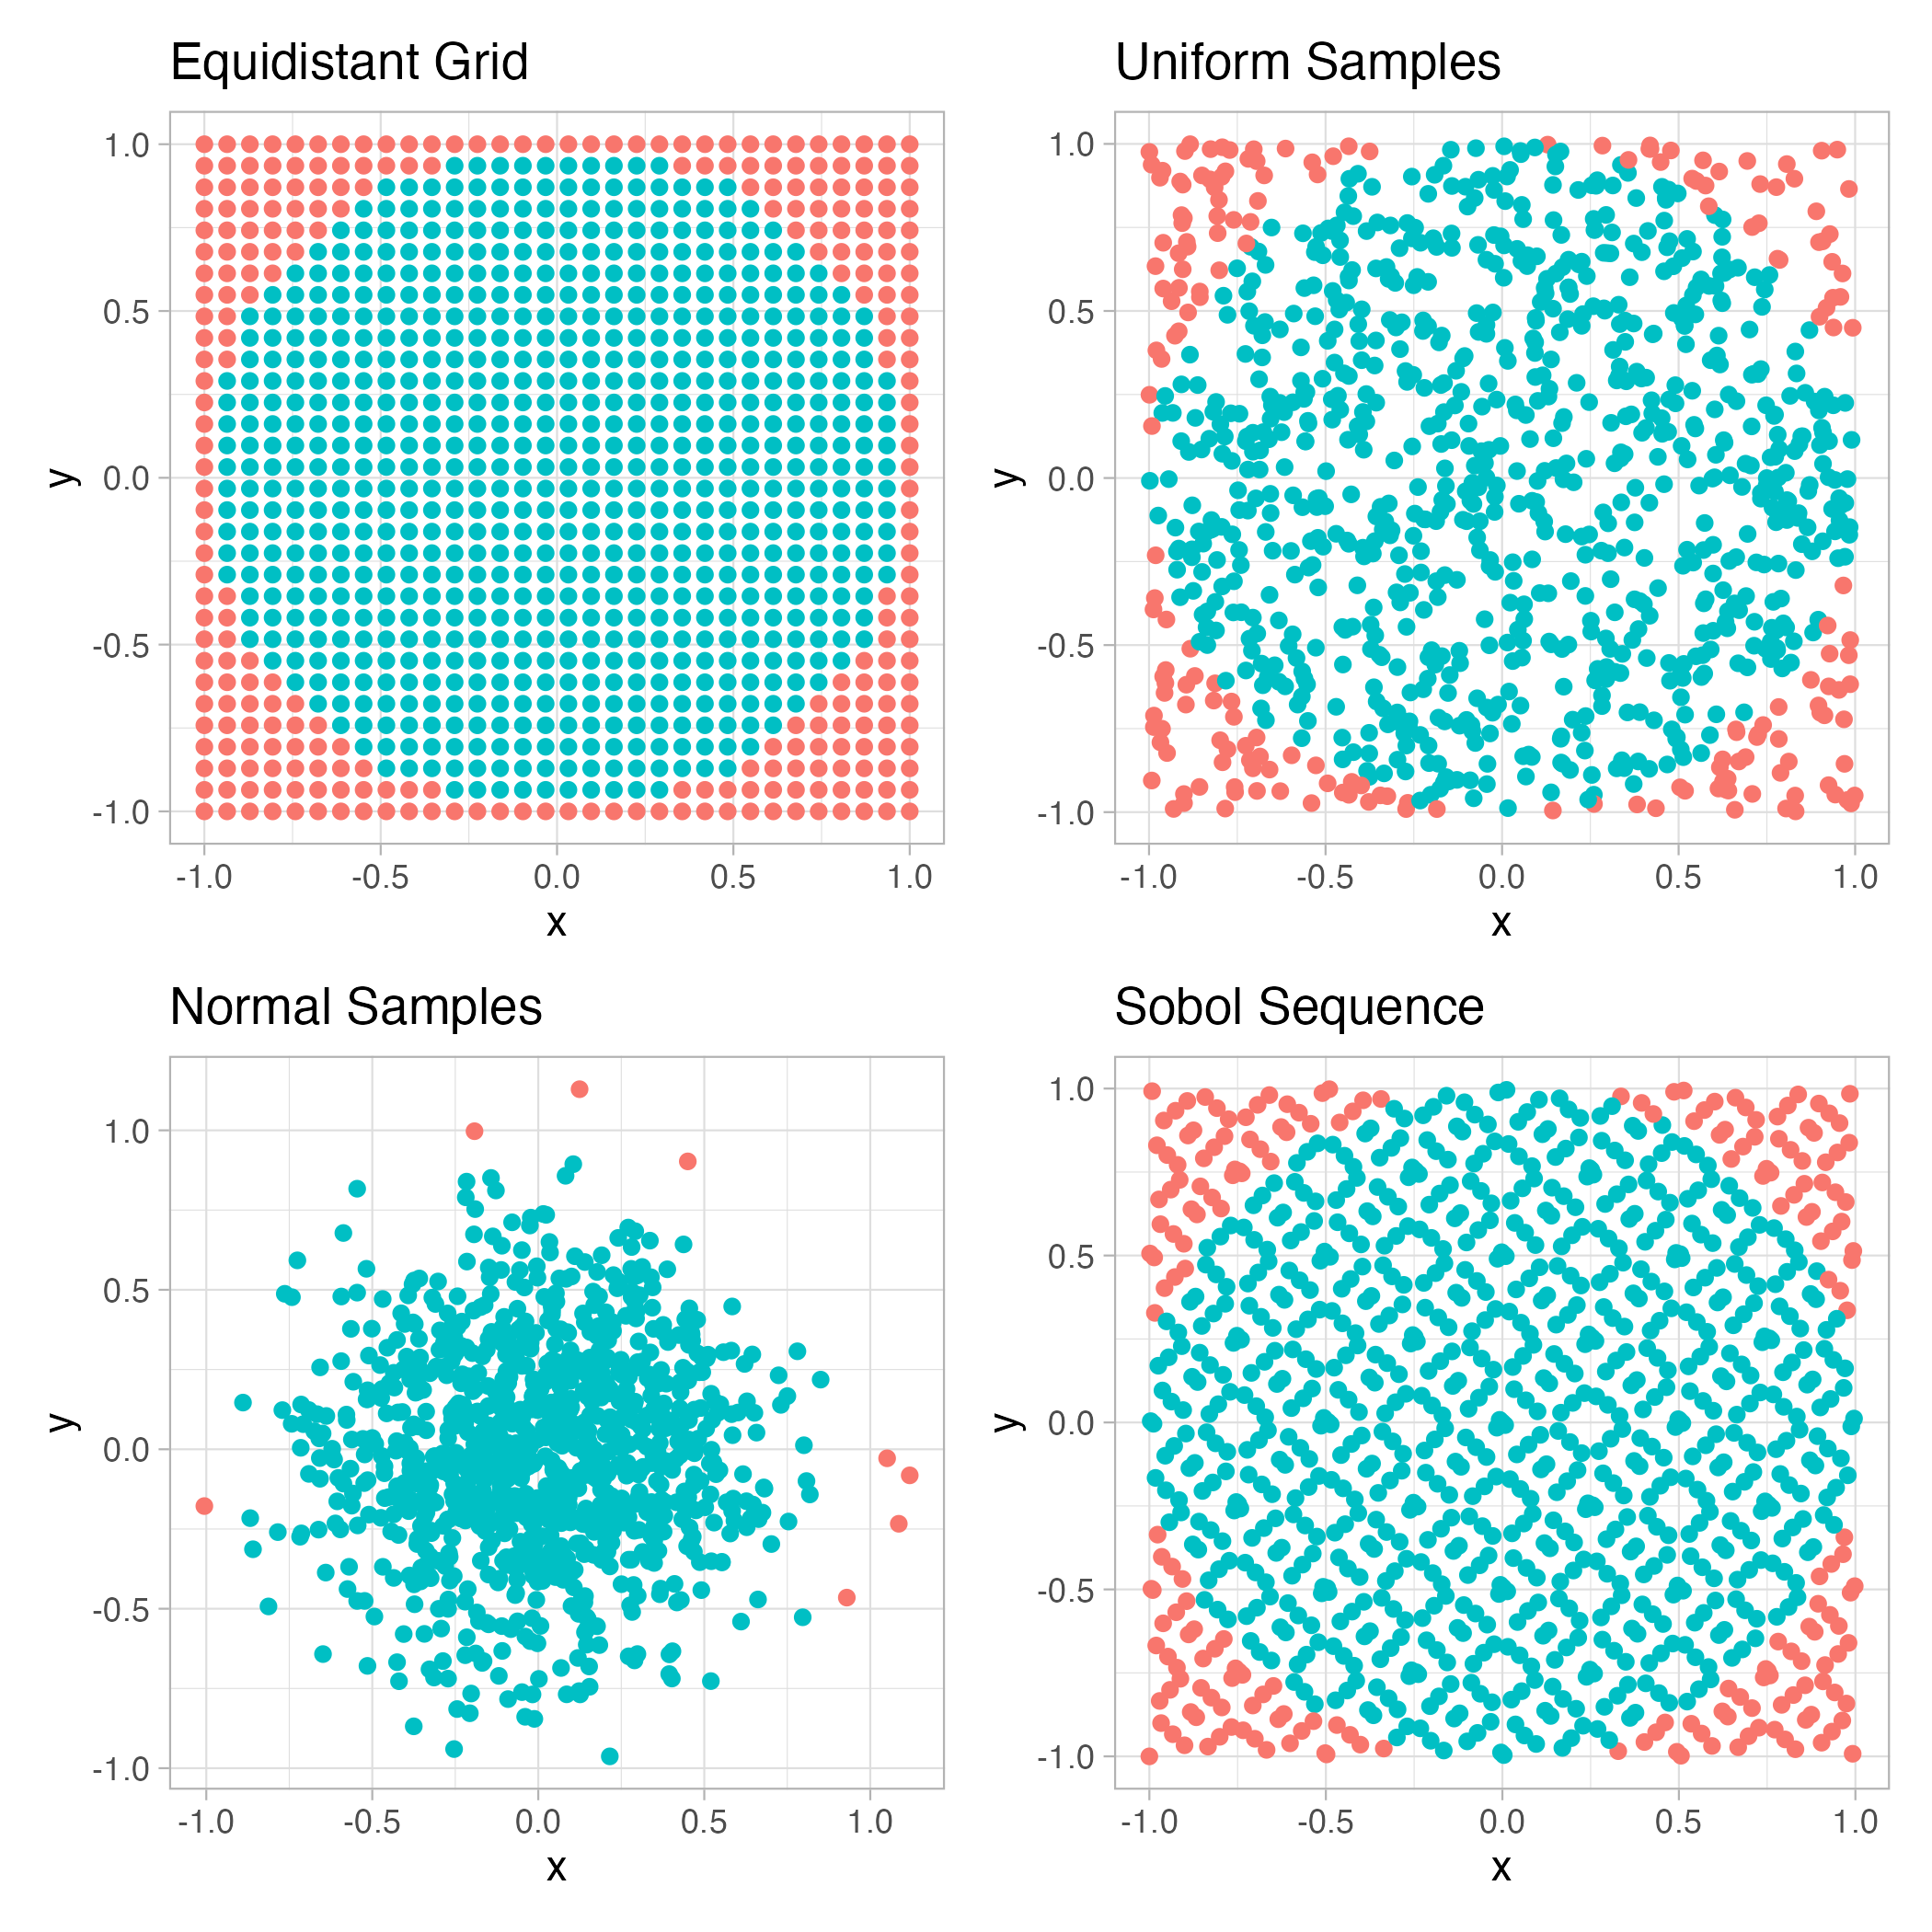
\includegraphics[width=\textwidth]{figures/ex1-samples.png}
        \caption{Visualization of the four sampling strategies, each with $2^{10} = 1024$ points colored by whether they fall inside the unit circle.}
        \label{fig:ex1-samples}
    \end{subfigure}
    \hfill
    \begin{subfigure}[b]{0.48\textwidth}
        \centering
        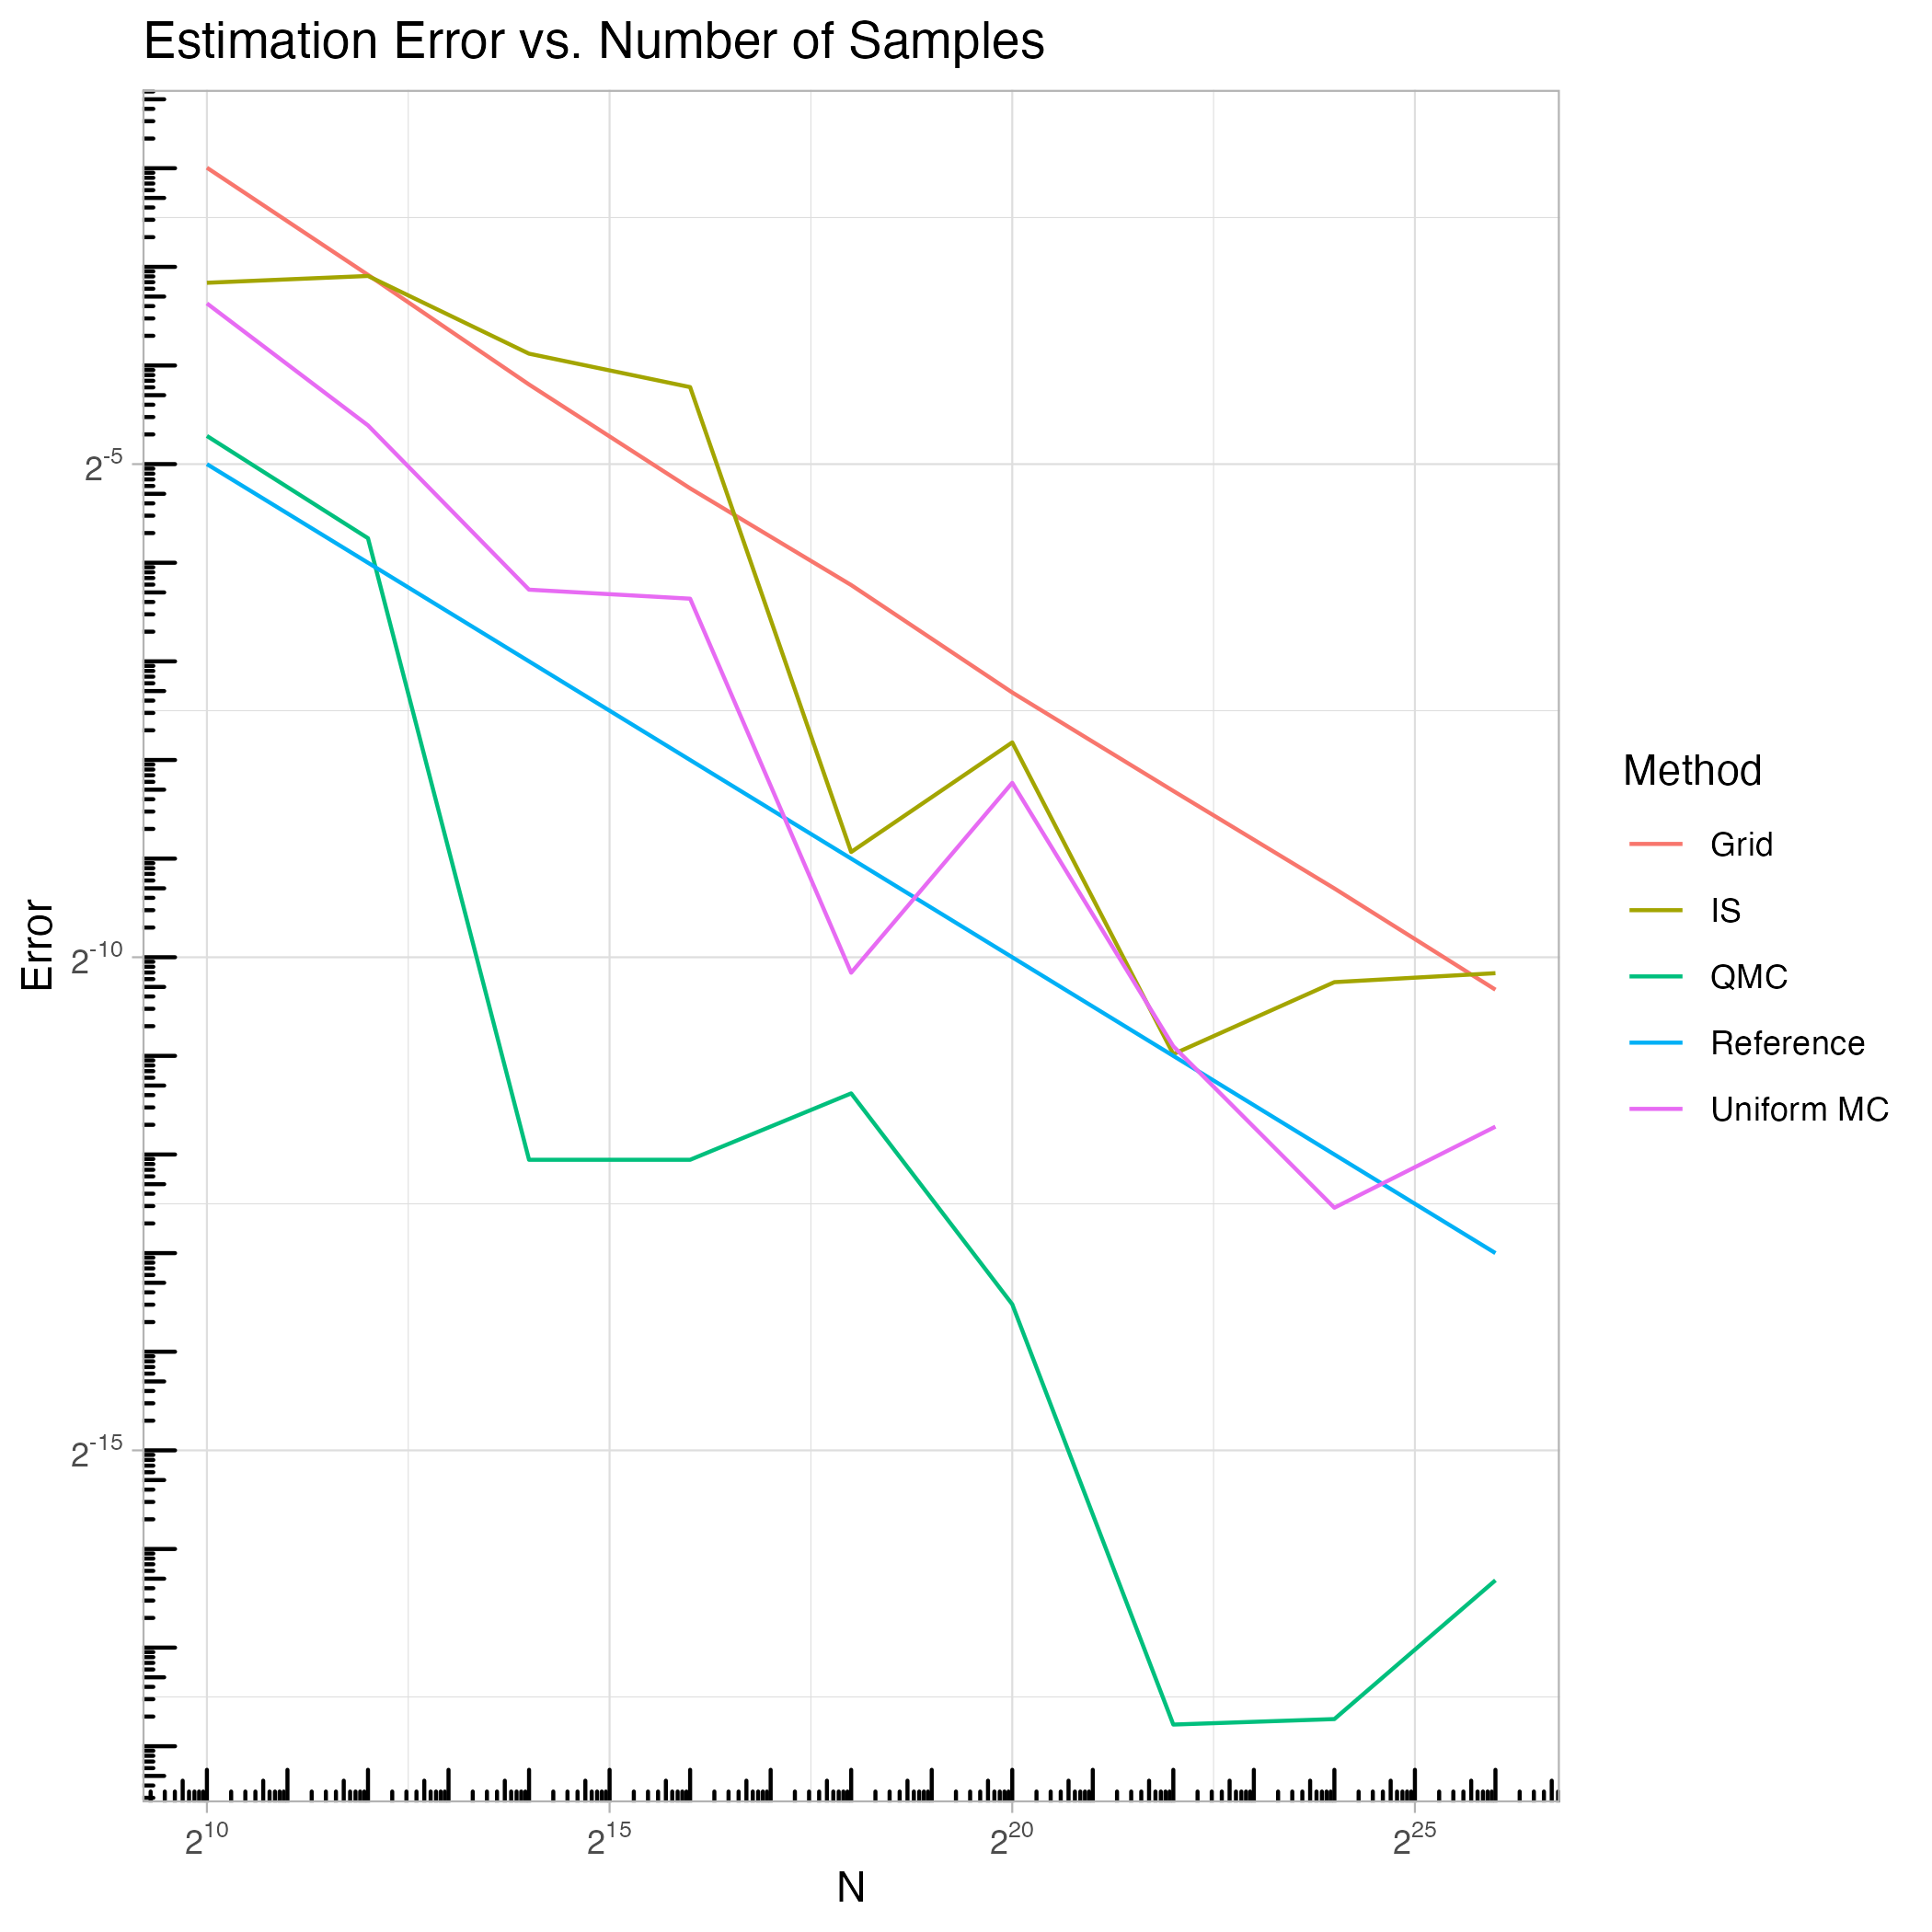
\includegraphics[width=\textwidth]{figures/ex1-estimation-error.png}
        \caption{Convergence comparison showing absolute error versus sample size. Sobol sequences demonstrate superior performance due to space-filling properties.}
        \label{fig:ex1-estimation-error}
    \end{subfigure}
    \caption{Comparison of sampling strategies for $\pi$ estimation. Generated using \href{https://github.com/NikoGerman/Seminar/blob/main/Notebooks/example1-estimating-pi.Rmd}{\texttt{example1-estimating-pi.Rmd}}.}
    \label{fig:pi-estimation-comparison}
\end{figure}

\textbf{Key Results:} Figure~\ref{fig:pi-estimation-comparison} shows that Sobol sequences demonstrate superior performance with consistently lower errors due to space-filling properties. Uniform Monte Carlo exhibits the expected $O(N^{-1/2})$ convergence, while the chosen importance sampling parameters provide no variance reduction for this problem.

\subsection{Probability of Rare Events}
\label{rare-events}

Estimating probabilities of rare events presents a fundamental challenge for standard Monte Carlo methods due to high variance and poor convergence. 
We demonstrate this challenge through a portfolio risk model where we estimate the probability of a remarkably high profit. In the following, we will discuss only the general setup and key results.
A comprehensive analysis of this problem, including theoretical background and implementation details, can be found at \href{https://nikogerman.github.io/Seminar/Notebooks/example2-rare-event.html}{\texttt{example2-rare-event.html}}. 

\textbf{Portfolio Setup:} Consider a portfolio with initially equally weighted assets, where each stock's log-return follows $Z_i \sim \mathcal{N}(\mu_i, \sigma_i^2)$ with parameters $\boldsymbol{\mu} = (-0.1, 0.2, -0.3, 0.1, 0)$ and $\boldsymbol{\sigma}^2 = (0.3, 0.3, 0.3, 0.2, 0.2)$. The portfolio value is $S = \sum_{i=1}^5 \exp(Z_i)$. Our objective is to estimate $\mathbb{P}(\bar{S} > 4)$, representing a 300\% profit.

\textbf{Methods Compared:} Standard Monte Carlo samples directly from the original distributions, while importance sampling uses shifted parameters $\tilde{\mu}_i = 1$ and $\tilde{\sigma}_i = 1$ to make the rare event more likely, then corrects using importance weights.

\textbf{Key Result:} For this rare event with probability $P \approx 2.3 \times 10^{-6}$, importance sampling achieves dramatically lower relative errors compared to standard Monte Carlo, enabling practical estimation of tail probabilities, as demonstrated in Figure \ref{fig:rare-events-analysis}.

\begin{figure}[h]
    \centering
    \begin{subfigure}[b]{0.48\textwidth}
        \centering
        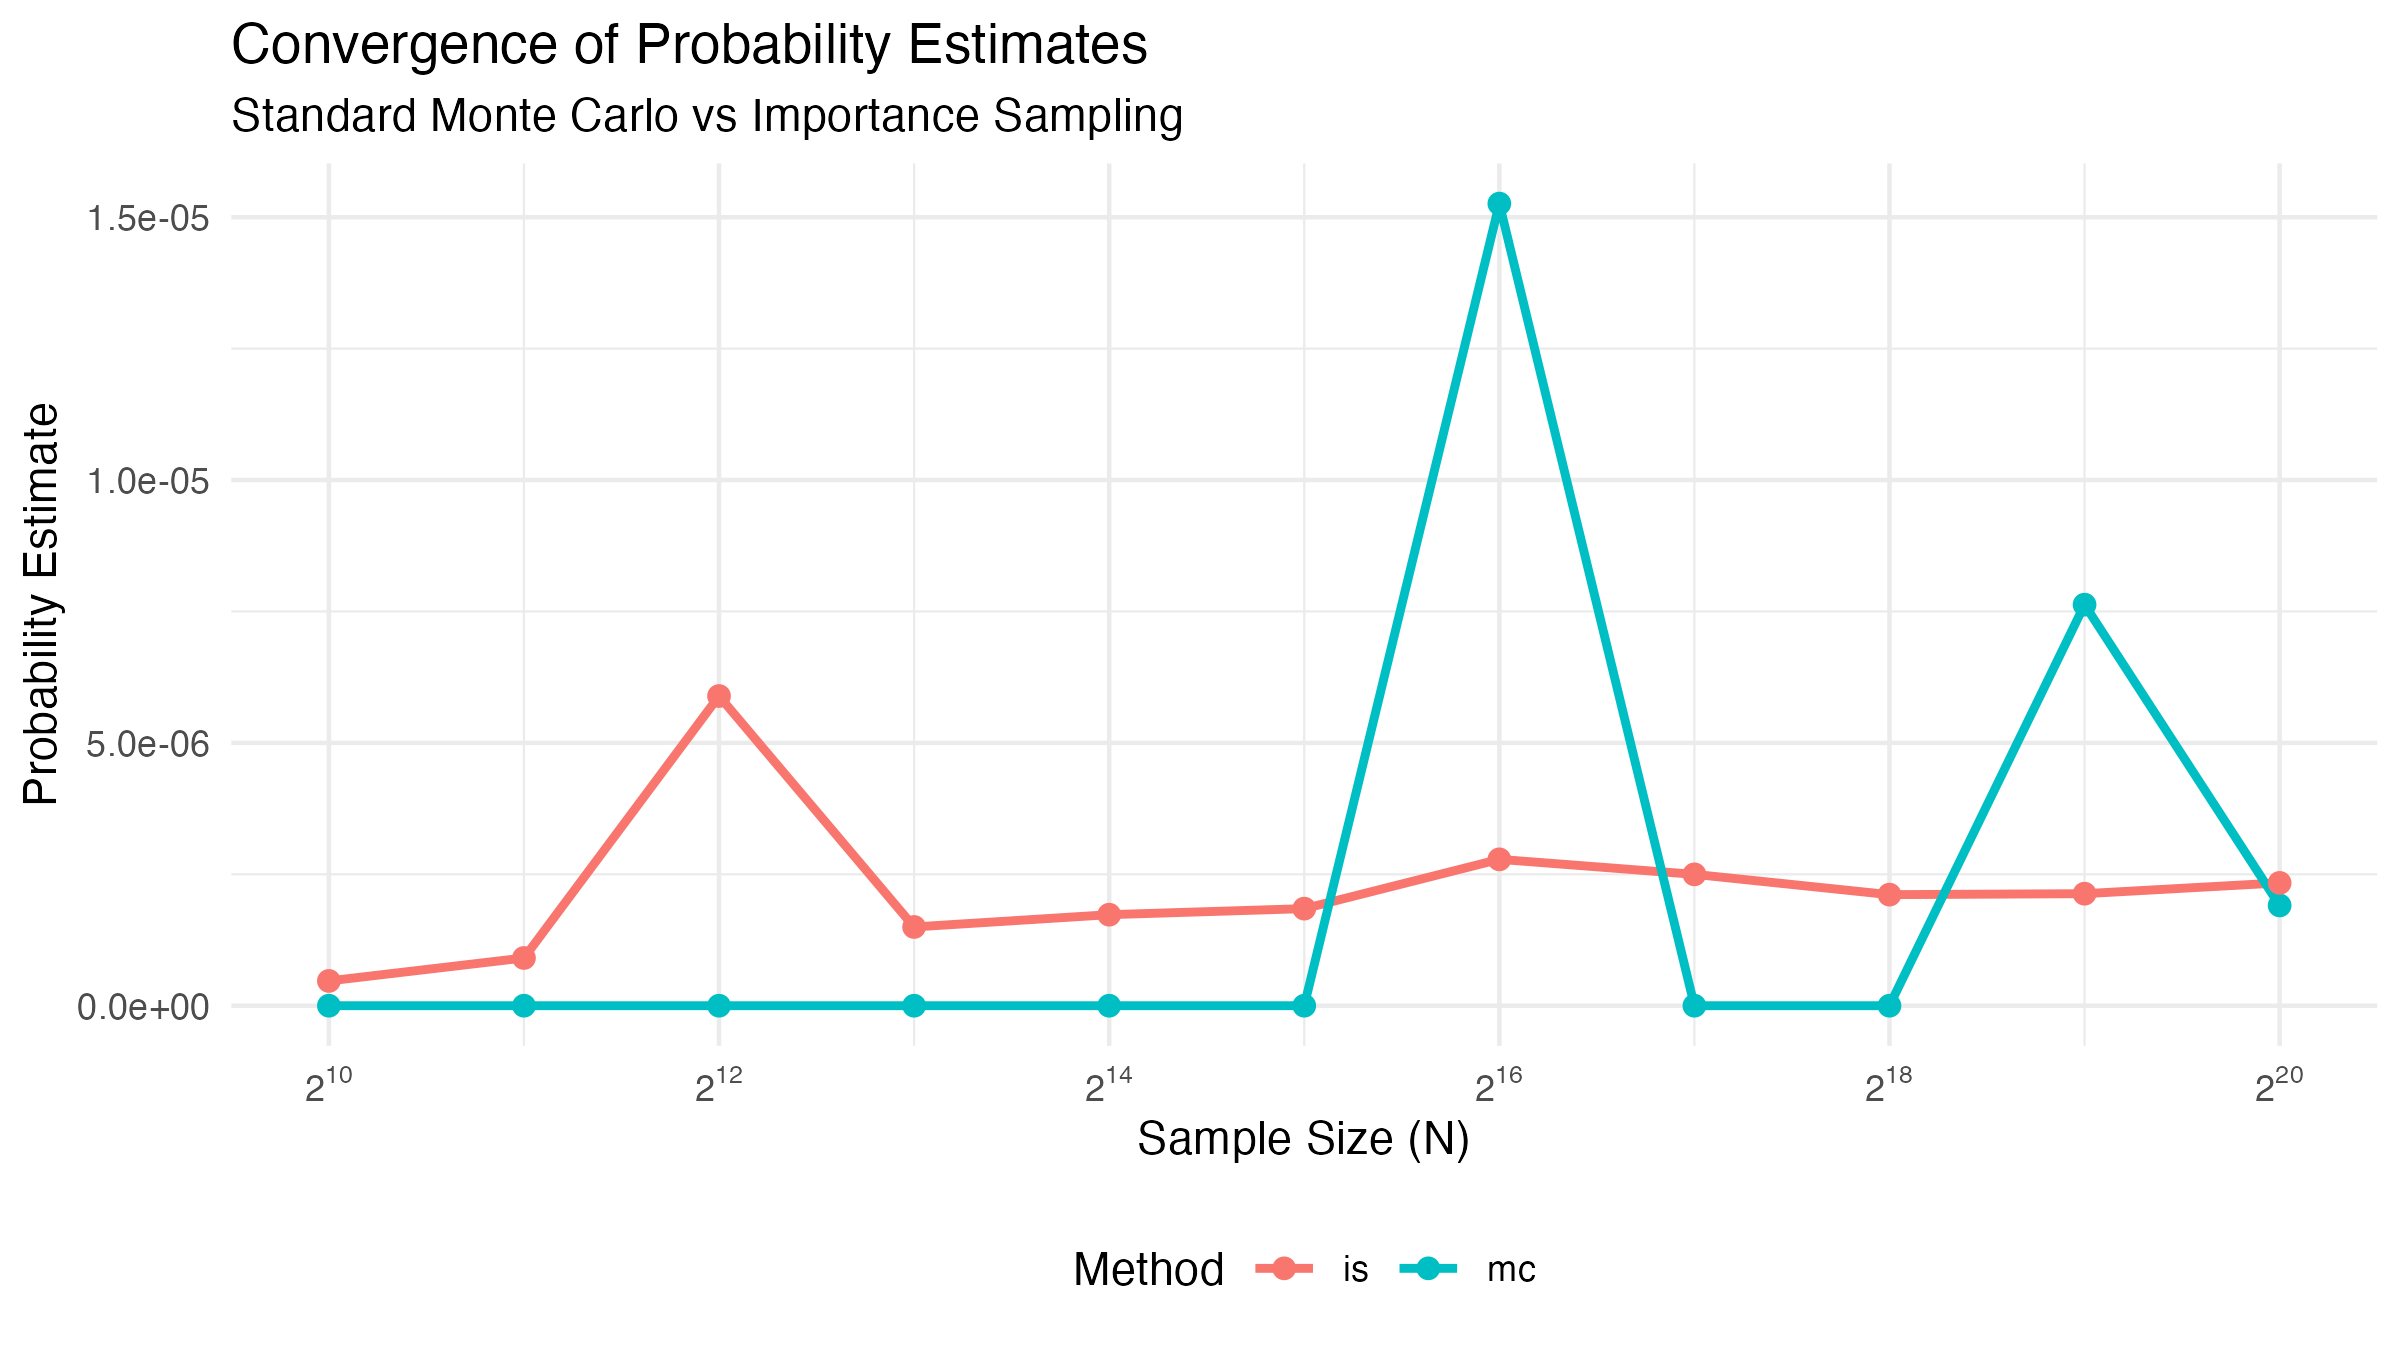
\includegraphics[width=\textwidth]{figures/ex2-estimates.png}
        \caption{Probability estimates versus sample size showing the superior convergence of importance sampling.}
        \label{fig:rare-events-estimates}
    \end{subfigure}
    \hfill
    \begin{subfigure}[b]{0.48\textwidth}
        \centering
        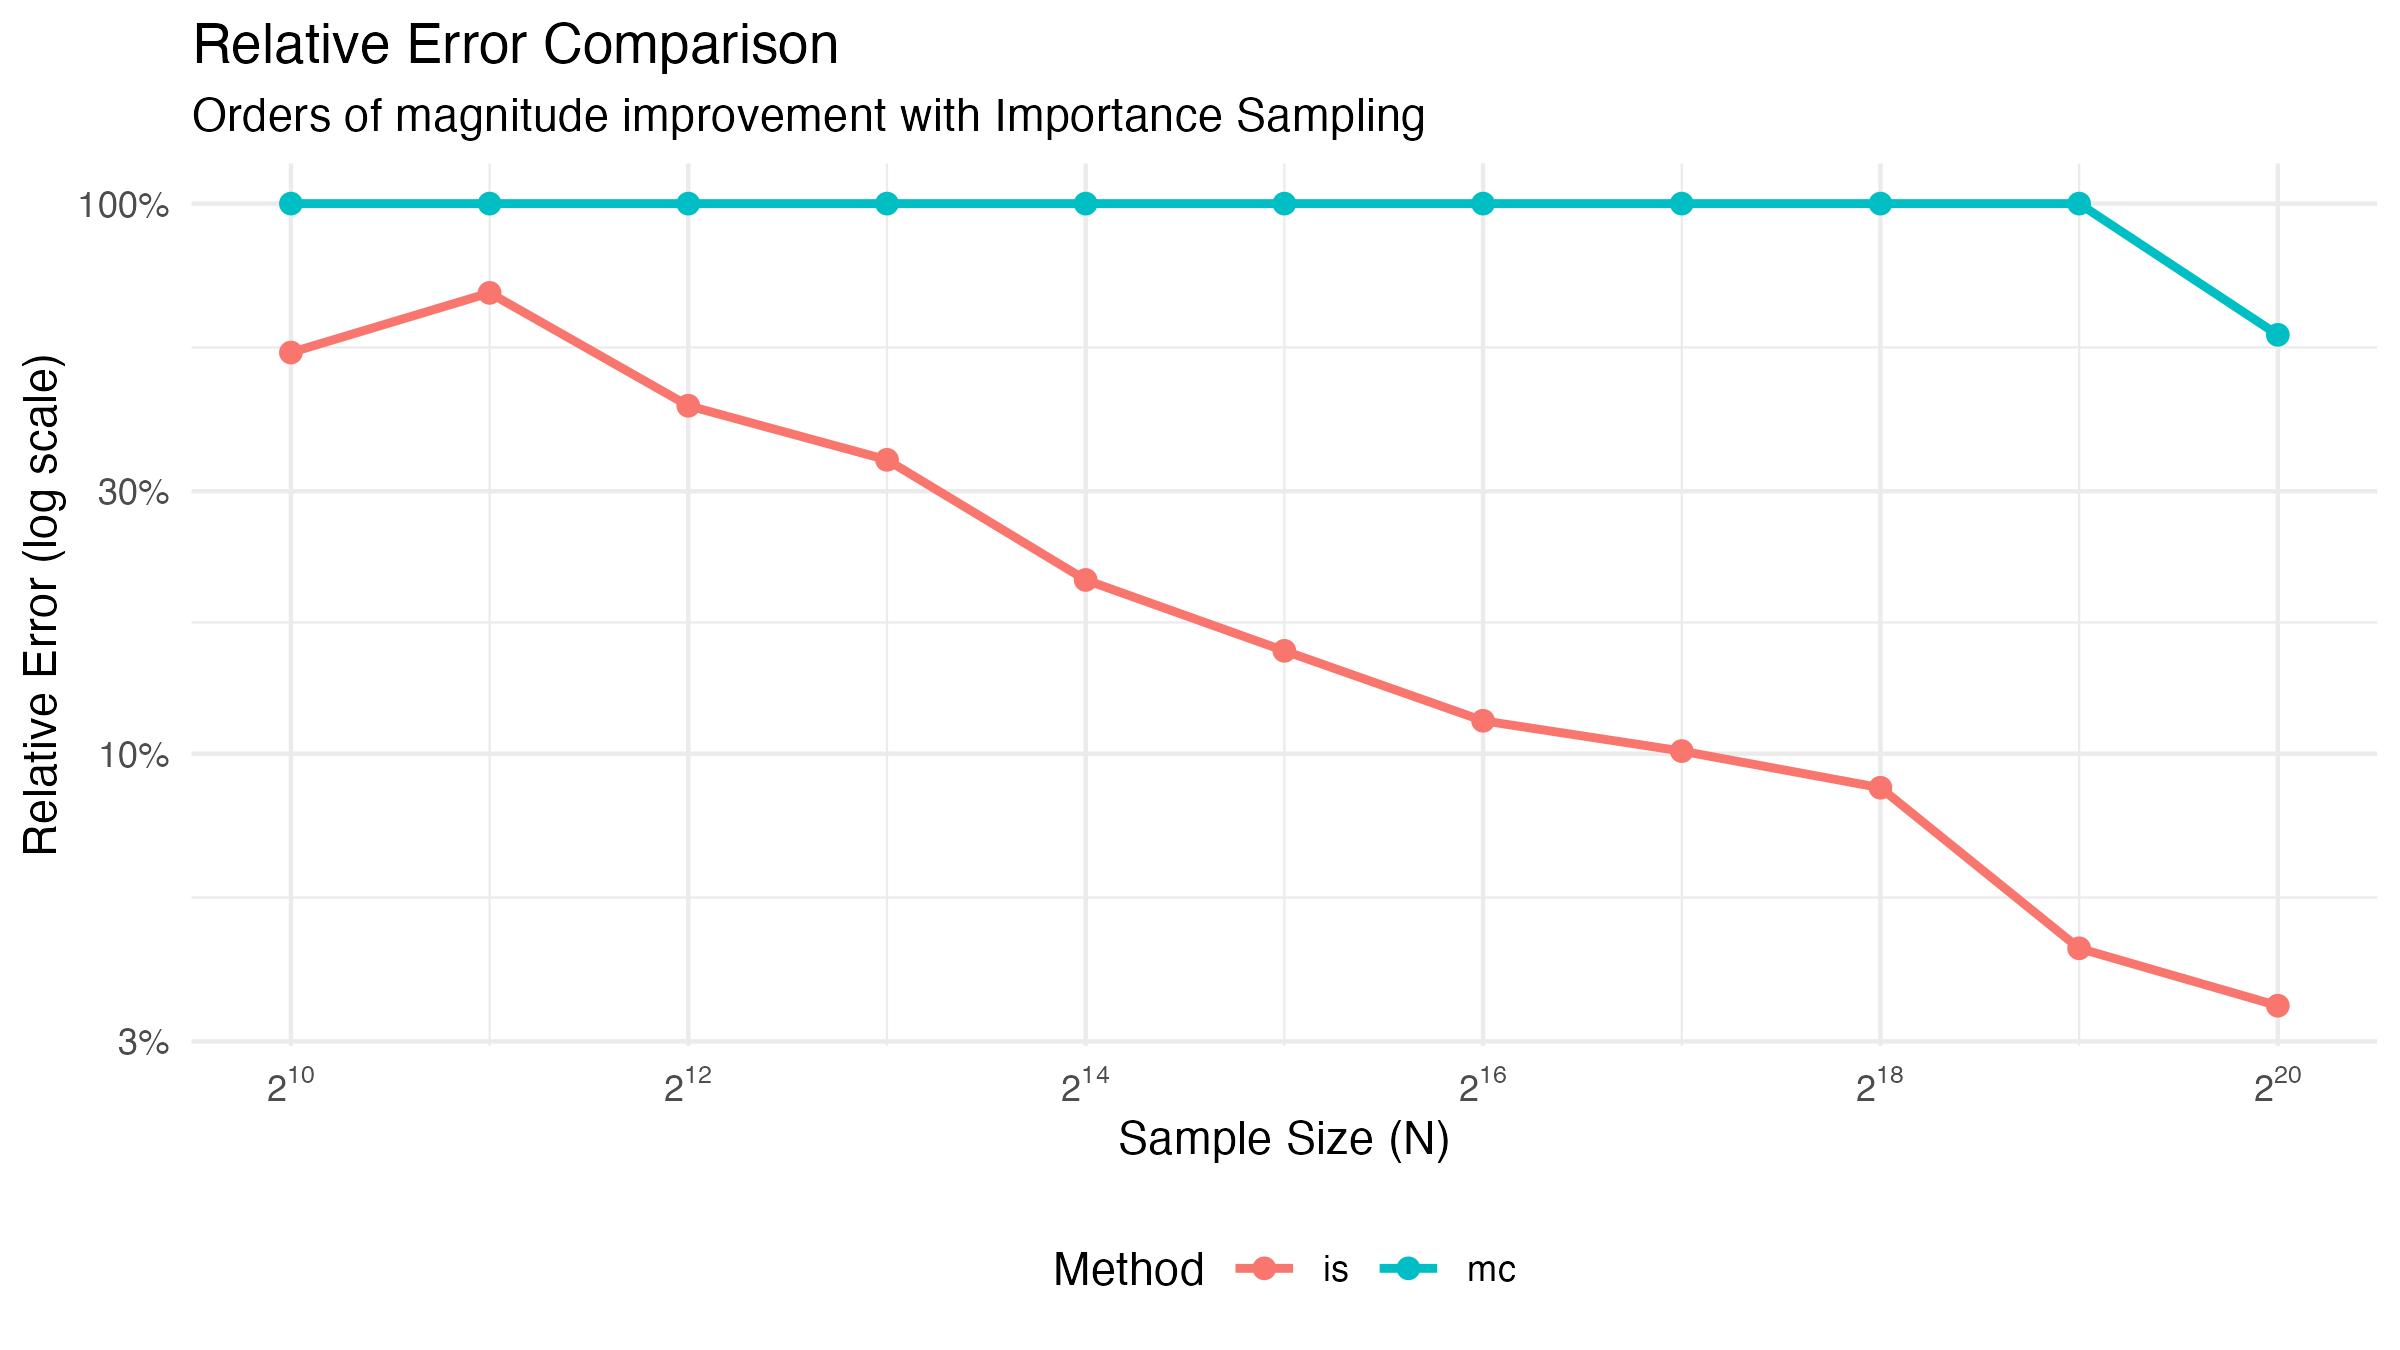
\includegraphics[width=\textwidth]{figures/ex2-rel-errors.png}
        \caption{Relative error comparison demonstrating orders of magnitude improvement with importance sampling.}
        \label{fig:rare-events-relative-errors}
    \end{subfigure}
    \caption{Comparison of standard Monte Carlo versus importance sampling for rare event estimation. Generated using \href{https://github.com/NikoGerman/Seminar/blob/main/Notebooks/example2-rare-event.Rmd}{\texttt{example2-rare-event.Rmd}}.}
    \label{fig:rare-events-analysis}
\end{figure}

This example illustrates why importance sampling is essential for applications requiring accurate tail probability estimation.

\section{Conclusion}
\label{conclusion}
The equivalence between integration and expectation forms the cornerstone of probabilistic Monte Carlo methods. This manifests in the identity $\mathbb{E}[\varphi(X)] = \int \varphi(x)f(x)dx$, which reveals that every expectation can be viewed as an integral and every integral can be recast as an expectation under an appropriate probability measure, thereby transforming the problem of numerical integration into one of statistical sampling. This insight allows deterministic integrals to be estimated by sample averages and provides the theoretical foundation for importance sampling and other variance reduction techniques. While quasi-Monte Carlo methods take a different approach through deterministic low-discrepancy sequences, both probabilistic and deterministic methods ultimately address the same fundamental challenge: efficient evaluation of high-dimensional integrals where traditional quadrature methods fail due to the curse of dimensionality.

\subsection{Advantages}
The primary strength of Monte Carlo methods lies in their dimension-independent convergence rate of $O(N^{-1/2})$, making them particularly valuable for high-dimensional problems that would be intractable through analytical or deterministic numerical approaches. This flexibility enables tackling complex integration problems across diverse domains. Monte Carlo methods naturally support variance reduction techniques such as importance sampling, which can significantly improve convergence rates. Furthermore, they provide natural uncertainty quantification through their inherent randomness, while quasi-Monte Carlo extensions can achieve even better convergence rates for smooth integrands.

\subsection{Limitations}
Monte Carlo methods face several fundamental limitations. The $O(N^{-1/2})$ convergence rate, while dimension-independent, is relatively slow compared to deterministic methods in low dimensions, and the stochastic nature introduces result variability. Many practical applications require sampling from complex or unknown distributions, necessitating advanced techniques like Markov Chain Monte Carlo or Sequential importance Sampling. Variance reduction techniques require domain expertise and can fail when poorly implemented. While quasi-Monte Carlo methods can overcome some limitations by achieving superior convergence rates, their deterministic nature prohibits confidence interval construction, eliminating natural uncertainty quantification.


\subsection{Outlook}
\label{outlook}
The field of Monte Carlo methods continues to evolve rapidly. An excellent source for recent advances is the biannual \textit{Monte Carlo and Quasi–Monte Carlo Methods} conference proceedings by Springer (\cite{plaskota_monte_2012}, \cite{dick_monte_2013}, \cite{cools_monte_2016}, \cite{owen_monte_2018}, \cite{tuffin_monte_2020}, \cite{keller_monte_2022}, \cite{hinrichs_monte_2024}).

\subsubsection{Sequential Importance Sampling}
\label{sis}
Sequential importance sampling extends static importance sampling to dynamic settings where the target distribution evolves over time or depends on sequential observations. This framework is particularly valuable in filtering problems for estimating posterior distributions of hidden states given sequential observations. For information on the method and statistical properties, \cite{murphy_probabilistic_2023, barbu_monte_2020} are excellent starting points.

\subsubsection{Markov Chain Monte Carlo}
\label{mcmc}
Markov Chain Monte Carlo methods enable sampling from complex multivariate distributions by constructing Markov chains with desired stationary distributions. MCMC methods, including Metropolis-Hastings algorithms and Gibbs sampling, make previously intractable posterior distributions accessible. \cite{barbu_monte_2020, murphy_probabilistic_2023} provide comprehensive treatments of MCMC and its applications. Recent developments include Hamiltonian Monte Carlo and variational inference.






\newpage
    
% ------------------------------------------------------------------------------
% BIBLIOGRAPHY -----------------------------------------------------------------
% ------------------------------------------------------------------------------

\RaggedRight
\bibliography{bibliography}
\bibliographystyle{dcu}
\newpage

% ------------------------------------------------------------------------------
% DECLARATION OF AUTHORSHIP-----------------------------------------------------
% ------------------------------------------------------------------------------


\Large
\noindent
\textbf{Declaration of authorship} 
\vspace{0.5cm}
\noindent
\normalsize

I hereby declare that the report submitted is my own unaided work. All direct 
or indirect sources used are acknowledged as references. I am aware that the 
Thesis in digital form can be examined for the use of unauthorized aid and in 
order to determine whether the report as a whole or parts incorporated in it may 
be deemed as plagiarism. For the comparison of my work with existing sources I 
agree that it shall be entered in a database where it shall also remain after 
examination, to enable comparison with future Theses submitted. Further rights 
of reproduction and usage, however, are not granted here. This paper was not 
previously presented to another examination board and has not been published.
\\

\vspace{1cm}
Munich, July 6, 2025

\vspace{3cm}

\noindent\rule{0.5\textwidth}{0.4pt} \\
Nikolai German

% ------------------------------------------------------------------------------
\newpage


% ------------------------------------------------------------------------------
% AI USAGE -----------------------------------------------------
% ------------------------------------------------------------------------------

\Large
\noindent
\textbf{Usage of Artificial Intelligence} 
\vspace{0.5cm}
\noindent
\normalsize

In the preparation of this paper, I utilized two Artificial Intelligence (AI) tools:

\begin{itemize}
    \item \textbf{Claude Sonnet 4}: Primarily used for proofreading draft chapters and improving readability and narrative flow. It was also used for LaTeX formatting tasks. Additionally, Claude was responsible for the complete implementation of the HTML index page that accompanies the paper, including all HTML/CSS/JavaScript code.
    
    \item \textbf{DeepL}: Used for proofreading chapter drafts and generating alternative formulations and explanations for individual text passages.
\end{itemize}


% ------------------------------------------------------------------------------
\newpage

% ------------------------------------------------------------------------------
% APPENDIX ---------------------------------------------------------------------
% ------------------------------------------------------------------------------
    
\pagenumbering{Roman}

\setcounter{page}{1} % CHANGE

\appendix

\section{Appendix}
\label{app}
\subsection{Mathematical Foundations}
\label{appendix:probability-theory}

This section provides essential mathematical concepts.

\subsubsection{Probability Theory}

\paragraph{Central Limit Theorem and Law of Large Numbers}
\label{appendix:clt}

The Strong Law of Large Numbers provides the fundamental justification for Monte Carlo methods. If $X_1, X_2, \ldots$ are independent and identically distributed random variables with finite mean $\mu$, then:
\begin{equation*}
    \bar{X}_n = \frac{1}{n}\sum_{i=1}^n X_i \xrightarrow{a.s.} \mu \quad \text{as } n \to \infty
\end{equation*}

The Central Limit Theorem establishes the rate of convergence and enables uncertainty quantification. For the same sequence with finite variance $\sigma^2$:
\begin{equation*}
    \bar{X}_n \xrightarrow{d} \mathcal{N}(\mu, \sigma^2/n) \quad \text{as } n \to \infty
\end{equation*}


\paragraph{Bivariate Change of Variables}
\label{appendix:change_of_vars}

For a bijective transformation $(Y_1,Y_2) = T(X_1,X_2)$ with inverse $H = T^{-1}$, the joint PDF transforms as:
\begin{equation*}
    f_{Y_1,Y_2}(y_1,y_2) = f_{X_1,X_2}(H(y_1,y_2)) \left|J_H(y_1,y_2)\right|
\end{equation*}

where $\left|J_H(y_1,y_2)\right|$ is the absolute determinant of the Jacobian matrix of $H$. This transformation rule is essential for deriving sampling methods like the Box-Muller transform.

\paragraph{Rayleigh Distribution}
\label{appendix:rayleigh}

The Rayleigh distribution with scale parameter $\sigma > 0$ has PDF:

\begin{equation*}
    f(x; \sigma) = 
        \begin{cases}
        \frac{x}{\sigma^2} \exp\left(\frac{-x^2}{2\sigma^2}\right) & x \geq 0\\
        0 & x < 0
    \end{cases}
\end{equation*}


and CDF:

\begin{equation*}
    F(x; \sigma) = 
        \begin{cases}
        1 - \exp\left(\frac{-x^2}{2\sigma^2}\right) & x \geq 0\\
        0 & x < 0
    \end{cases}
\end{equation*}

The Rayleigh distribution is related to the exponential distribution: if $X \sim \text{Exp}(\lambda)$, then $\sqrt{X} \sim \text{Rayleigh}\left(\frac{1}{\sqrt{2\lambda}}\right)$.

\subsubsection{Linear Algebra}
\label{appendix:linear-algebra}

\paragraph{Positive Definite Matrices and Cholesky Decomposition}
\label{appendix:Cholesky}

A symmetric matrix $\Sigma \in \mathbb{R}^{d \times d}$ is positive definite if $x^T\Sigma x > 0$ for all non-zero vectors $x \in \mathbb{R}^d$. Every positive definite matrix admits a unique Cholesky decomposition $\Sigma = LL^T$, where $L$ is lower triangular with positive diagonal entries.

\subsection{Computational Methods}
\label{appendix:computational-methods}

This section covers computational techniques for implementing Monte Carlo methods.

\subsubsection{Low Discrepancy Sequences}
\label{appendix:low_discrepancy}

Low discrepancy sequences provide deterministic point sets with superior uniformity compared to pseudo-random sequences. The discrepancy of a sequence $P = \{x_1, \ldots, x_N\}$ in $[0,1)^d$ measures deviation from uniformity:
\begin{equation*}
D(P, \mathcal{F}) = \sup_{B \in \mathcal{F}} \left| \frac{\#(B \cap P)}{N} - \text{vol}(B) \right|
\end{equation*}
where $\mathcal{F}$ is typically a family of rectangular test sets.

\textbf{Sobol sequences} are particularly effective in moderate to high dimensions and widely used in financial applications. \textbf{Halton sequences} are simpler to generate and perform well in low dimensions, but quality deteriorates in higher dimensions due to coordinate correlations.

While standard Monte Carlo achieves $\mathcal{O}(N^{-1/2})$ convergence, low discrepancy sequences can achieve $\mathcal{O}((\log N)^d/N)$ for smooth integrands—a significant improvement in moderate dimensions, though the curse of dimensionality limits benefits as $d$ increases.

\subsubsection{Random Number Generation}
\label{appendix:rng}

The Lehmer generator provides a foundation for pseudo-random number generation using the recurrence $X_{n+1} = (a \cdot X_n) \bmod m$. A standard implementation uses multiplier $a = 7^5$ and modulus $m = 2^{31} - 1$:

\begin{algorithm}
\caption{Lehmer Random Number Generator}\label{algo:lehmer-rng}
\begin{algorithmic}
    \Require $X_0 > 0$ \Comment{Initial seed}
    \State $a \gets 7^5, $m \gets 2^{31} - 1$
    \State $X \gets X_0$
    \Loop
        \State $X \gets (a \cdot X) \bmod m$
        \State $U \gets X / m$ \Comment{Convert to uniform on $(0,1)$}
        \State \Return $U$
    \EndLoop
\end{algorithmic}
\end{algorithm}

The choice of parameters $a$ and $m$ is crucial for achieving good statistical properties and full period length (see \cite{lemieux_monte_2009}).

\subsection{Algorithms}
\label{appendix:algos}

\begin{algorithm}
\caption{Box-Muller Transform}\label{algo:box-muller}
\begin{algorithmic}
    \State $U_1, U_2 \gets$ \Call{runif\_01}{2} \Comment{Generate two uniform random variables}
    \State $R \gets \sqrt{-2 \ln(U_1)}$ \Comment{Transform to radius}
    \State $\Theta \gets 2\pi U_2$ \Comment{Transform to angle}
    \State $X_1 \gets R \cos(\Theta)$ \Comment{First standard normal sample}
    \State $X_2 \gets R \sin(\Theta)$ \Comment{Second standard normal sample}
    \State \Return $(X_1, X_2)$
\end{algorithmic}
\end{algorithm}

\begin{algorithm}
\caption{Acceptance-Rejection Sampling}\label{algo:acceptance-rejection}
\begin{algorithmic}
    \Repeat
        \State $\tilde{X} \gets$ \Call{rand\_r()}{} \Comment{Sample from density $r(x)$}
        \State $U \gets$ \Call{runif\_01}{1} \Comment{Generate uniform random variable}
        \State $\alpha \gets p(\tilde{X})/t(\tilde{X})$ \Comment{Calculate acceptance probability}
    \Until{$U \leq \alpha$} \Comment{Accept if $U$ falls below threshold}
    \State $X \gets \tilde{X}$ \Comment{Set accepted sample}
    \State \Return $X$
\end{algorithmic}
\end{algorithm}

\begin{algorithm}
\caption{Adaptive Rejection Sampling}
\label{algo:adaptive-rejection}
\begin{algorithmic}
    \Require $\log p(x)$ \Comment{Log-density of target distribution}
    \Require $T_0 = \{x_1, x_2, \ldots, x_k\}$ \Comment{Initial tangent points}
    \State $T \gets T_0$ \Comment{Initialize tangent point set}
    \State $E \gets$ \Call{construct\_envelope}{$T$} \Comment{Build initial envelope}
    \Loop
        \State $\tilde{X} \gets$ \Call{sample\_from\_envelope}{$E$} \Comment{Sample from current envelope}
        \State $U \gets$ \Call{runif\_01}{1} \Comment{Generate uniform random variable}
        \State $\alpha \gets \frac{p(\tilde{X})}{E(\tilde{X})}$ \Comment{Calculate acceptance ratio}
        \If{$U \leq \alpha$} \Comment{Accept sample}
            \State \Return $\tilde{X}$
        \Else \Comment{Reject and refine envelope}
            \State $T \gets T \cup \{\tilde{X}\}$ \Comment{Add rejected point to tangent set}
            \State $E \gets$ \Call{construct\_envelope}{$T$} \Comment{Rebuild envelope with new point}
        \EndIf
    \EndLoop
\end{algorithmic}
\end{algorithm}


\newpage


\section{Electronic appendix}
\label{el_app}

Data, code and figures can be found on \href{https://github.com/NikoGerman/Seminar}{\color{blue}github.com}.

\end{document}